% 中文版:
% \chapter{实现\label{chap:implementation}}
% 为了让读者能够完全复现该工程，在本章中，我们将详细介绍本工程的实现过程，包括硬件选择、环境搭建、软件开发等方面的内容。


% \section{环境搭建\label{sec:environment_setup}}
% 在本节中，我们将介绍如何搭建本工程所需的环境，包括PC机、Turtlebot3、 Jetson Orin Nano。

% \subsection{PC机\label{subsec:pc_setup}}
% 本工程使用的PC机为一台普通的笔记本电脑，具体硬件配置参见\autoref{tab:lenovo_laptop_specs}。在PC机上，主要安装操作系统、ROS 2、rtabmap功能包、本工程功能包\texttt{uoa_robot_drone}、开发环境VS Code并进行相应环境配置，下面我们将详细介绍这些步骤。
% \subsubsection{安装操作系统\label{subsubsec:os_setup}}
% 本工程使用的操作系统为Ubuntu 22.04 LTS。*注意：为了少出问题，务必使用\textbf{物理机直装}方式安装，不要使用虚拟机形式(虚拟机上的Ubuntu为Jetson Orin Nano刷机时经常失败)。安装步骤如下：
% \begin{enumerate}
%     \item 点击https://releases.ubuntu.com/22.04/该链接，如图~\ref{fig:download_ubuntu_desktop}所示，下载Ubuntu 22.04 LTS的ISO镜像文件。
%         \begin{figure}[htbp]
%             \centering
%             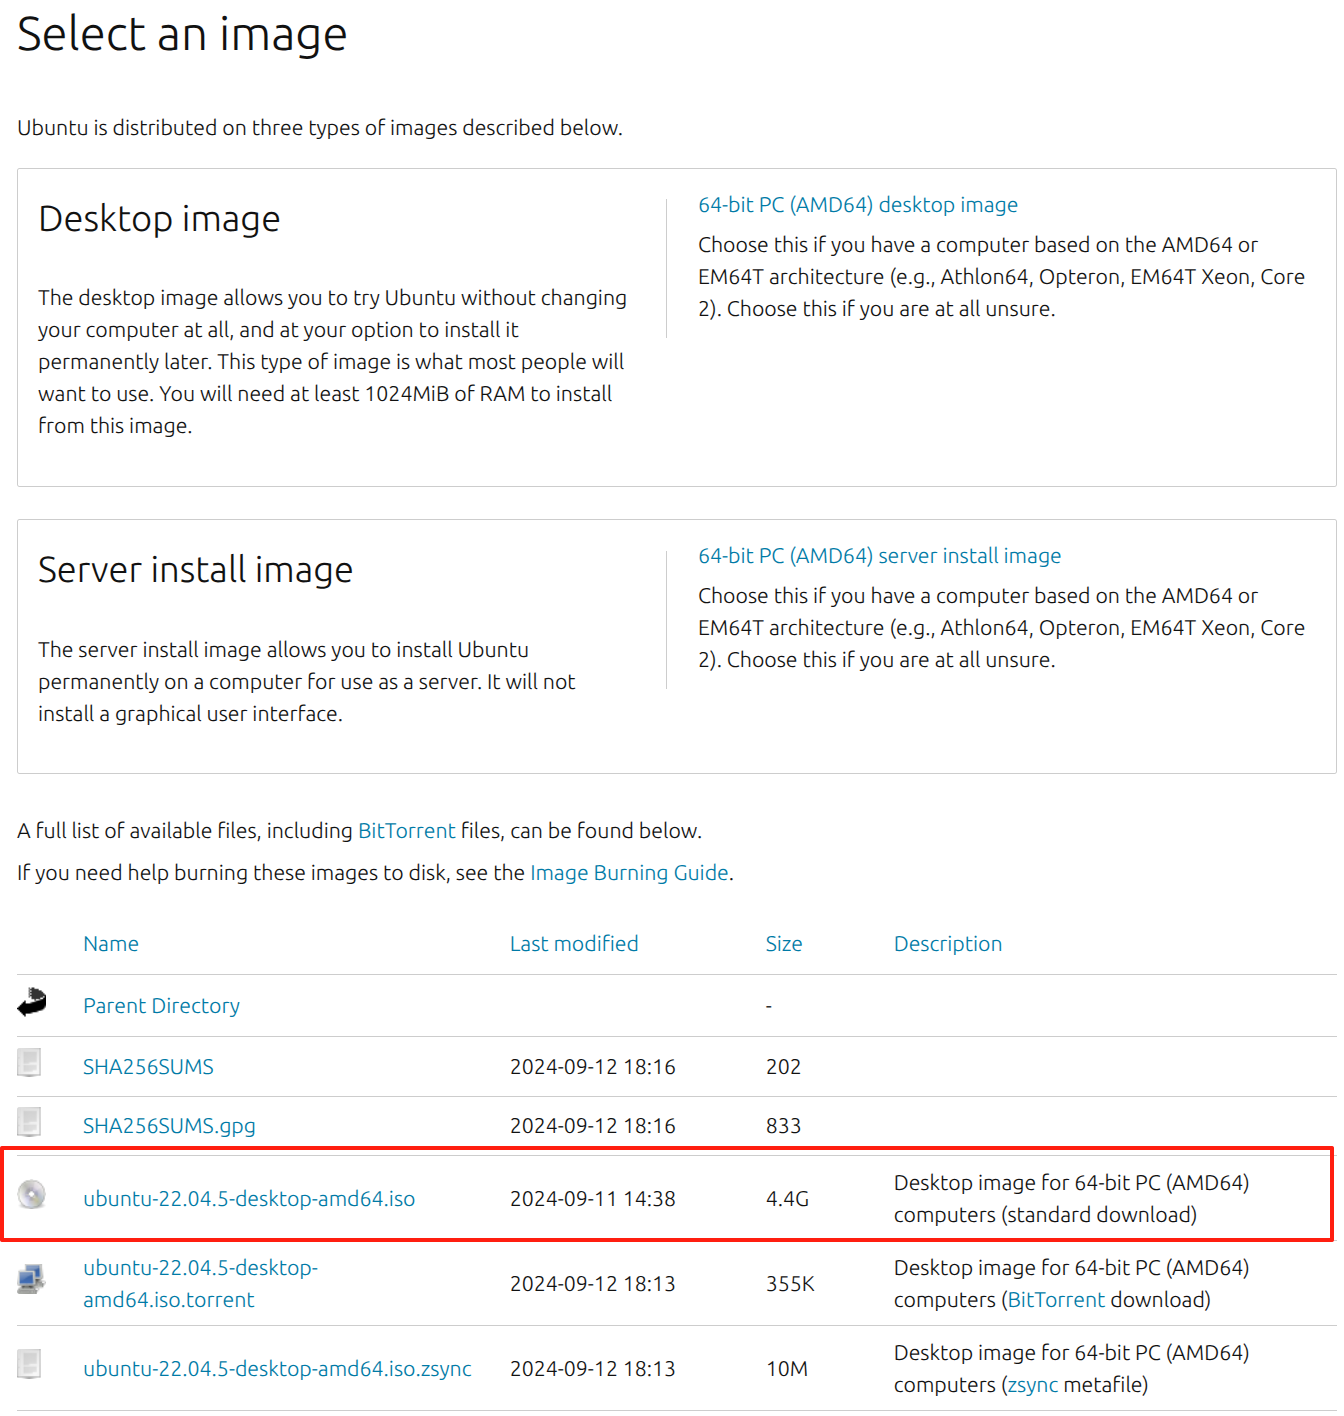
\includegraphics[width=0.9\textwidth]{figs/implementation/download_ubuntu_desktop.png}
%             \caption{下载Ubuntu 22.04 LTS的ISO镜像文件}
%             \label{fig:download_ubuntu_desktop}
%         \end{figure}
%     \item 如图所示，参照教程\href{https://ubuntu.com/tutorials/install-ubuntu-desktop#1-overview}{Install Ubuntu Desktop}完成OS的安装。
%         \begin{figure}[htbp]
%             \centering
%             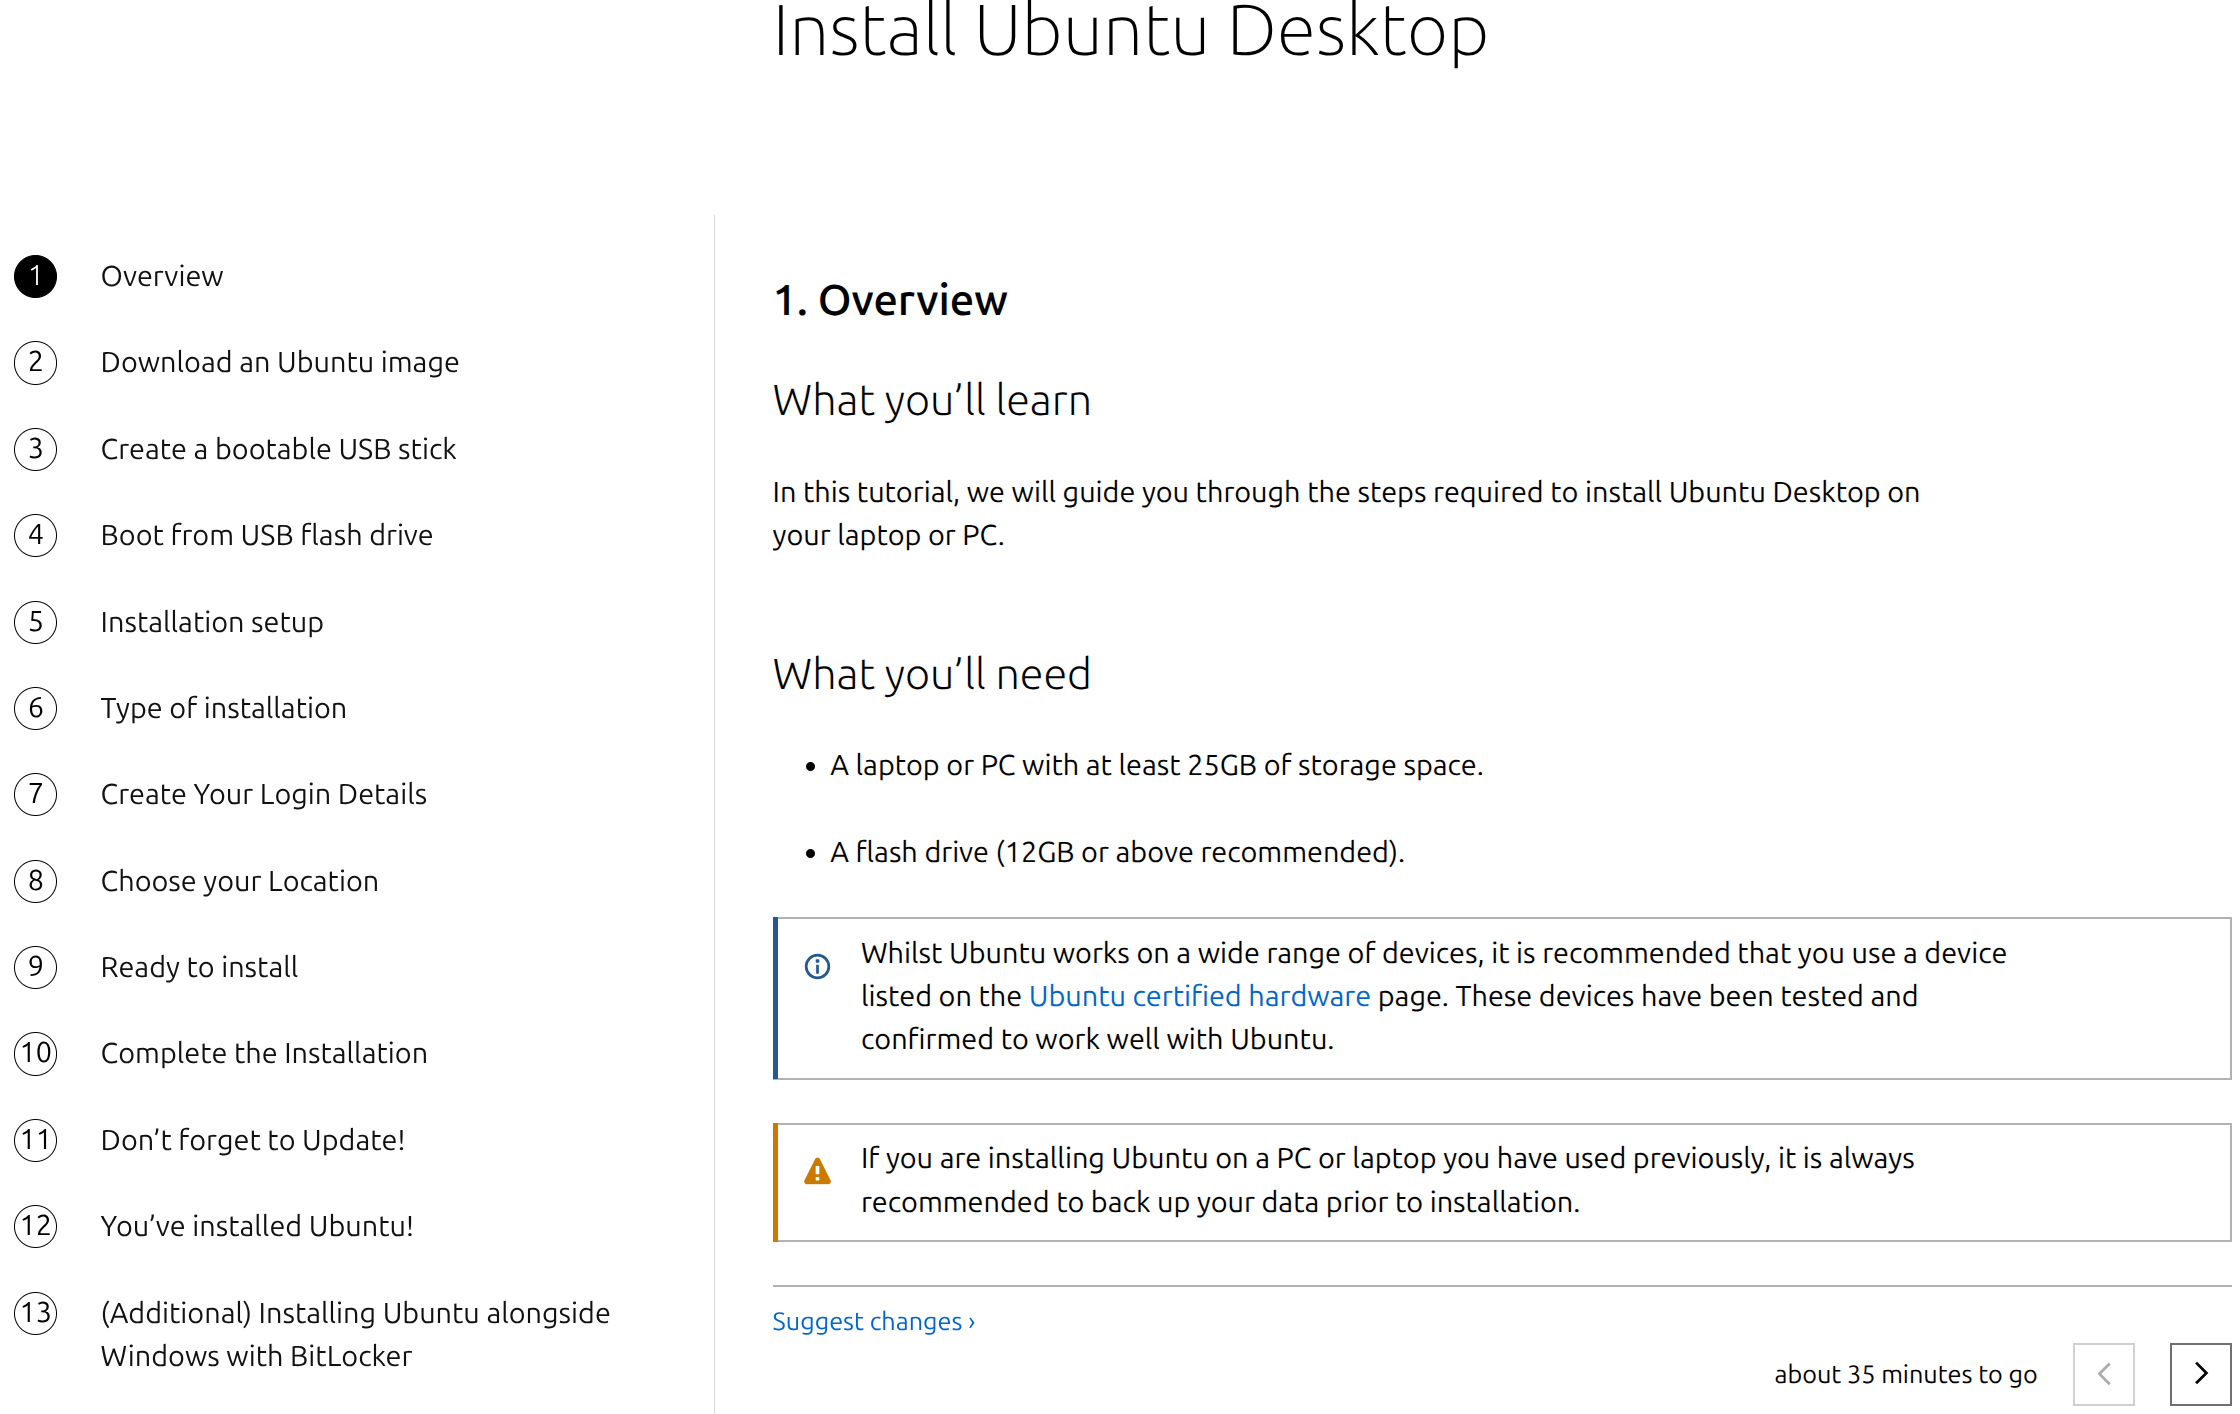
\includegraphics[width=0.9\textwidth]{figs/implementation/install_ubuntu_desktop.png}
%             \caption{安装Ubuntu 22.04 LTS}
%             \label{fig:install_ubuntu_desktop}
%         \end{figure}
% \end{enumerate}

% \subsubsection{安装ROS 2\label{subsubsec:ros_setup}}
% 本工程使用的ROS 2版本为Humble Hawksbill。按照教程\href{https://docs.ros.org/en/humble/Installation/Ubuntu-Install-Debs.html}{Ubuntu (deb packages)}逐步进行安装，执行完如图~\ref{fig:try_some_examples}所示的步骤即可。
% \begin{figure}[htbp]
%     \centering
%     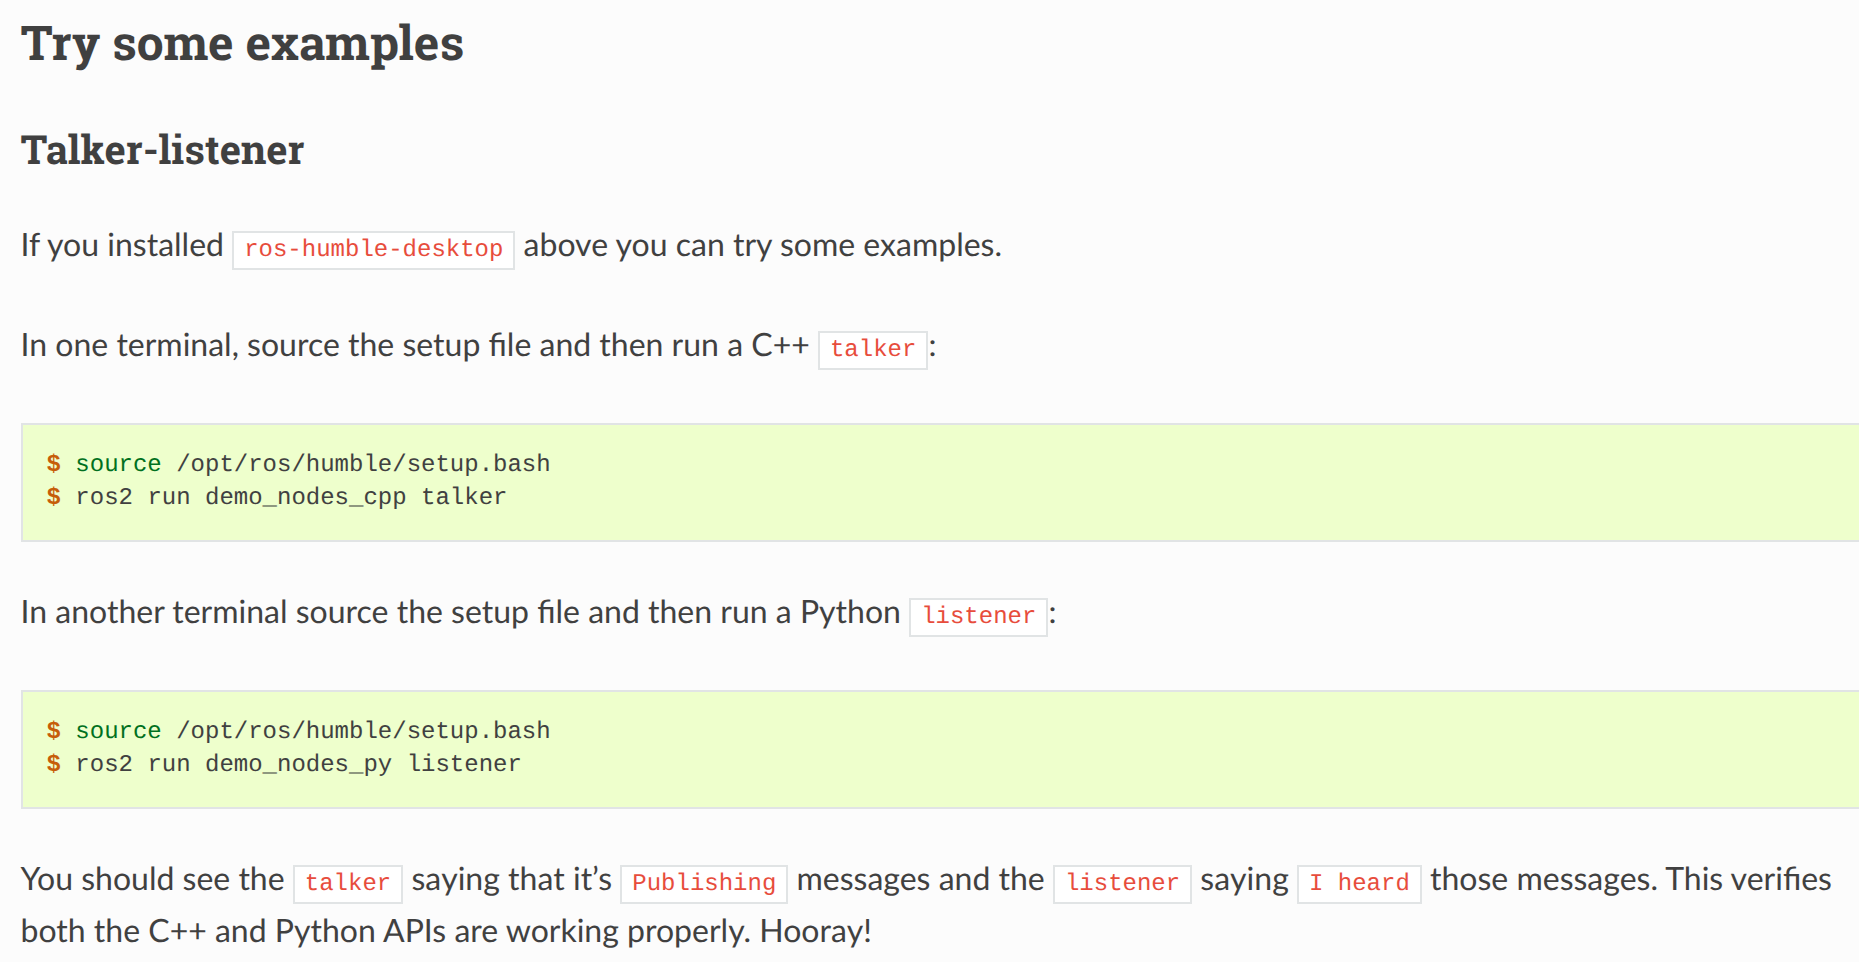
\includegraphics[width=0.9\textwidth]{figs/implementation/try_some_examples.png}
%     \caption{安装ROS 2 Humble Hawksbill}
%     \label{fig:try_some_examples}
% \end{figure}

% \subsubsection{安装功能包\label{subsubsec:packages_setup}}
% 在PC机上，本工程使用的功能包主要是Turtlebot3的、rtabmap的、navigation2的。
% [On PC] 相关安装命令如下：
% $ source /opt/ros/humble/setup.bash
% $ mkdir -p ~/ros2_ws/src
% $ cd ~/ros2_ws/src/
% $ git clone -b humble https://github.com/ROBOTIS-GIT/DynamixelSDK.git
% $ git clone -b humble https://github.com/ROBOTIS-GIT/turtlebot3_msgs.git
% $ git clone -b humble https://github.com/ROBOTIS-GIT/turtlebot3.git
% $ git clone https://github.com/introlab/rtabmap.git
% $ git clone -b ros2 https://github.com/introlab/rtabmap_ros.git
% $ git clone -b humble https://github.com/ros-navigation/navigation2.git
% $ git clone -b humble https://github.com/Jian-UOA/CS5917.git
% $ sudo apt install python3-colcon-common-extensions
% $ cd ~/ros2_ws
% $ colcon build --symlink-install

% \subsubsection{安装开发环境\label{subsubsec:dev_env_setup}}
% 本工程使用的开发环境为Visual Studio Code。安装步骤如下：
% \begin{enumerate}
%     \item 点击https://code.visualstudio.com/Download该链接，下载相应版本的Visual Studio (本工程中选的是x64), 如图~\ref{fig:download_vscode}所示。
%         \begin{figure}[htbp]
%             \centering
%             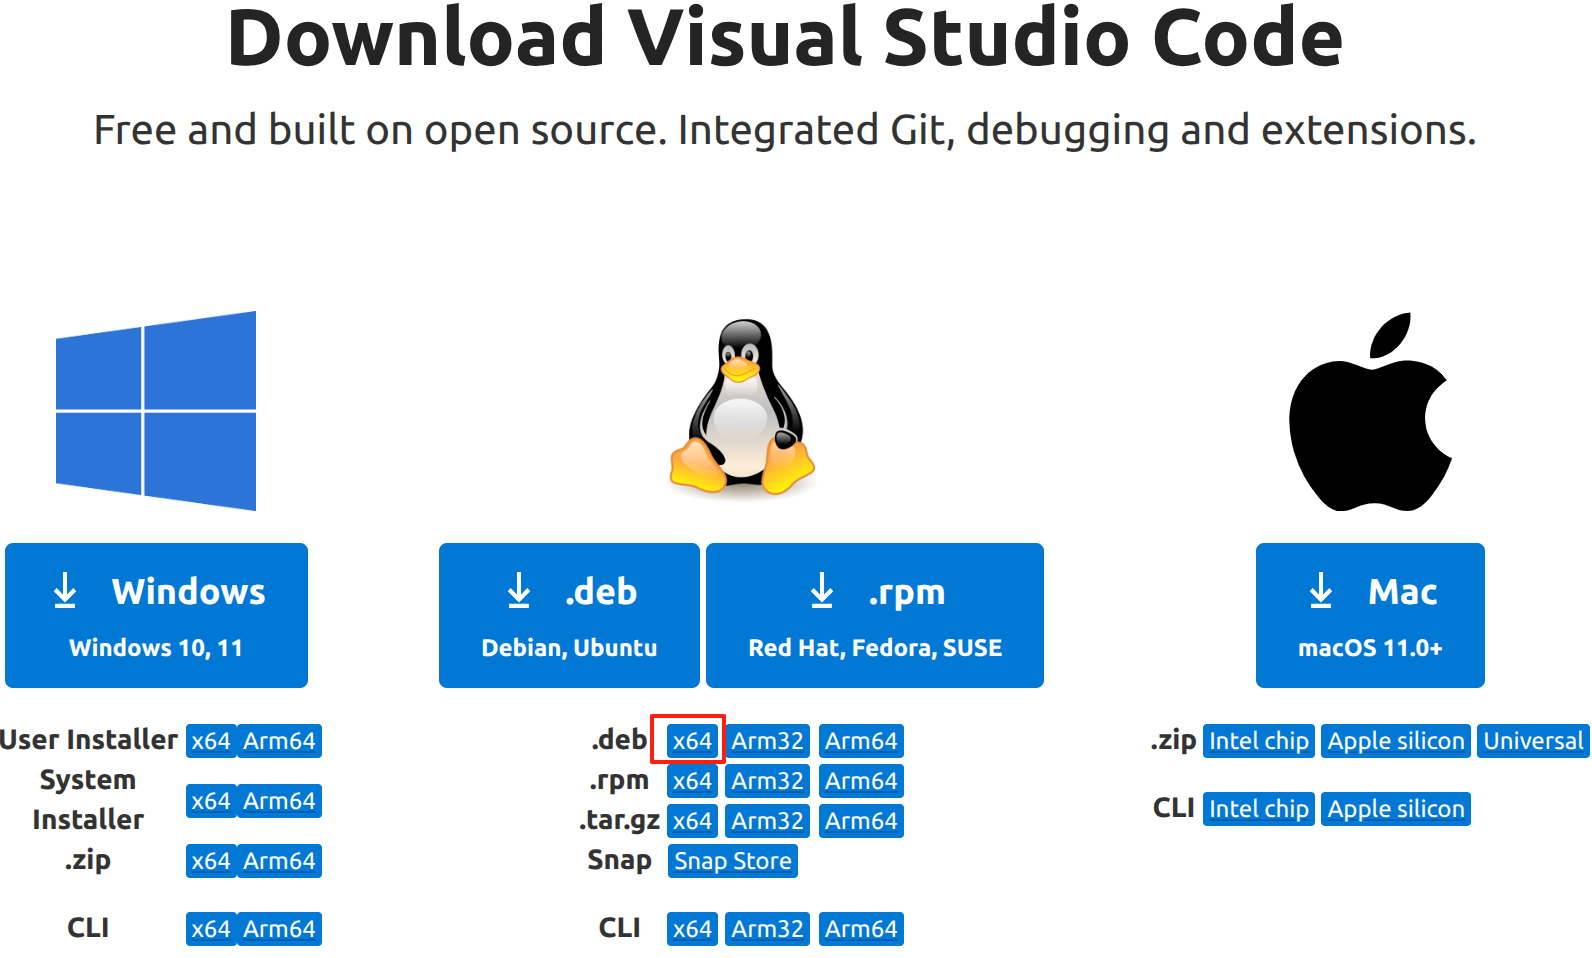
\includegraphics[width=0.9\textwidth]{figs/implementation/download_vscode.png}
%             \caption{下载Visual Studio Code}
%             \label{fig:download_vscode}
%         \end{figure}
%      \item 进入刚才下载文件的保存目录，找到下载的安装文件(\texttt{code_1.103.1-1755017277_amd64.deb})，按照教程\href{https://code.visualstudio.com/docs/setup/linux#_install-vs-code-on-linux}{Install VS Code on Linux}完成安装。如图~\ref{fig:install_vscode}所示。
%         \begin{figure}[htbp]
%             \centering
%             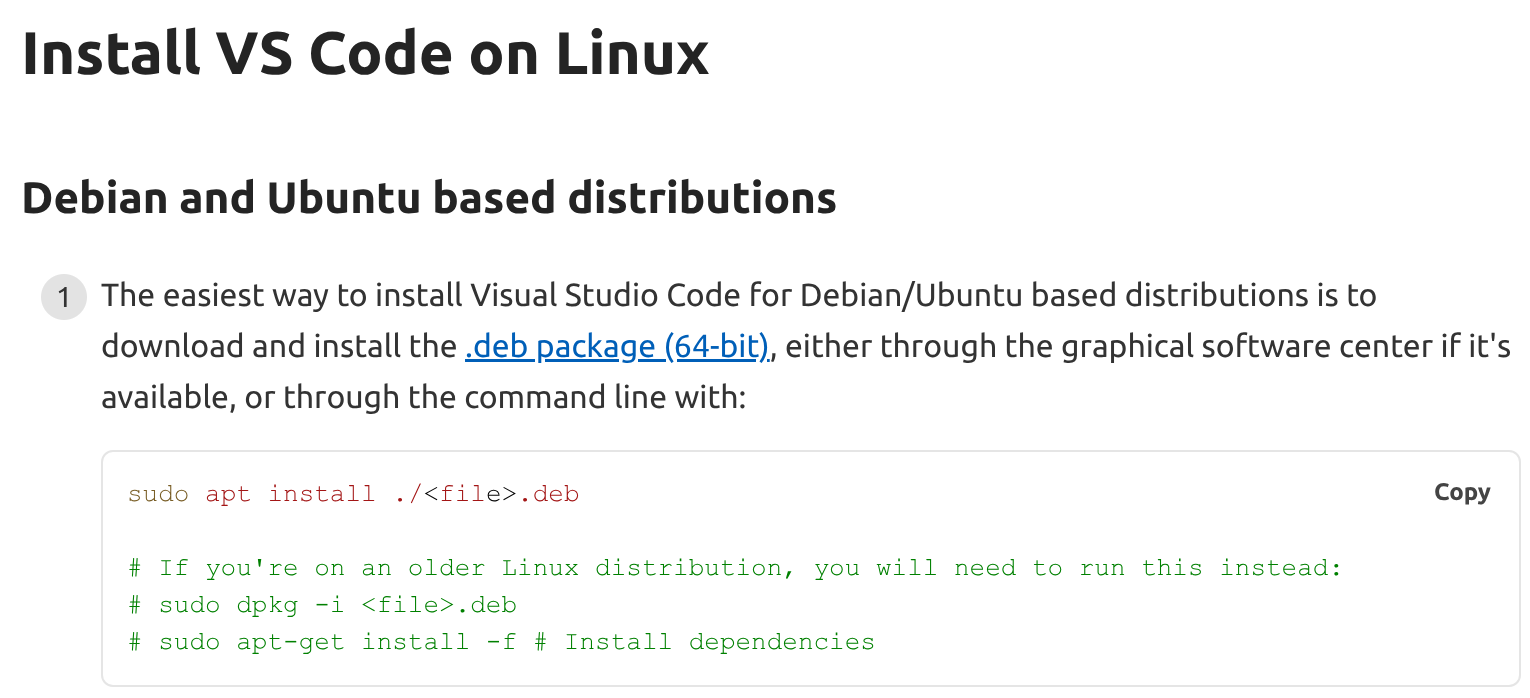
\includegraphics[width=0.9\textwidth]{figs/implementation/install_vscode.png}
%             \caption{安装Visual Studio Code}
%             \label{fig:install_vscode}
%         \end{figure}
%       \item 打开Visual Studio Code，按照教程\href{https://code.visualstudio.com/docs/getstarted/getting-started}{Tutorial: Get started with Visual Studio Code}中的示例，完成基本配置，打开目录\texttt{~/ros2_ws}中的工作空间，应该可以看到类似图~\ref{fig:open_ros2_ws}中的内容。
%         \begin{figure}[htbp]
%             \centering
%             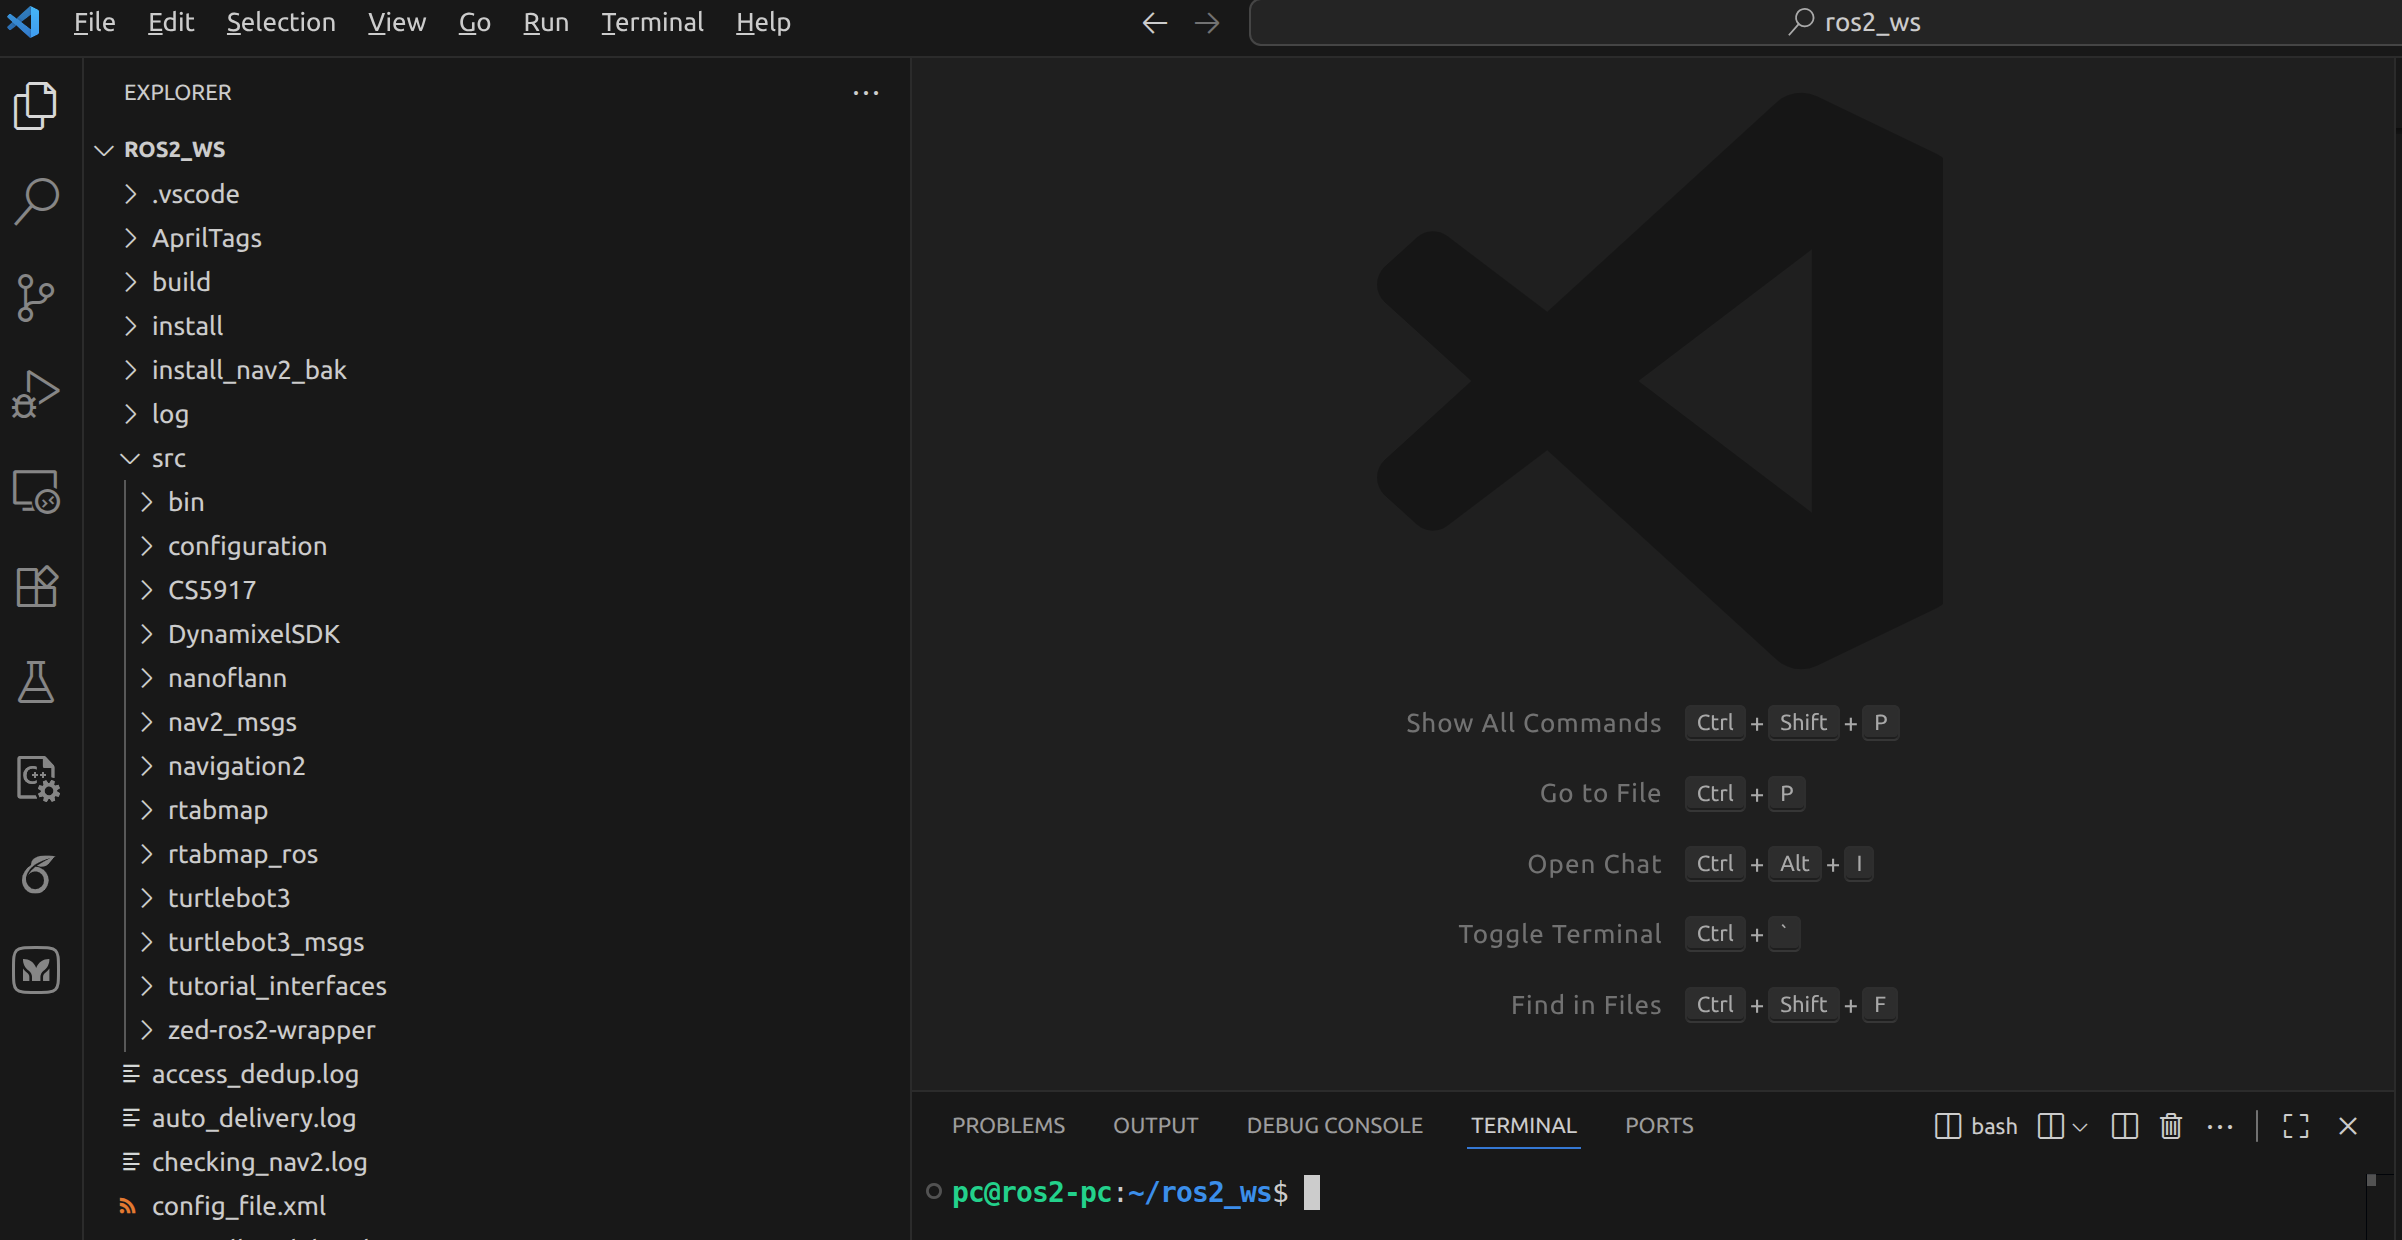
\includegraphics[width=0.9\textwidth]{figs/implementation/open_ros2_ws.png}
%             \caption{打开ROS 2工作空间}
%             \label{fig:open_ros2_ws}
%         \end{figure}
% \end{enumerate}

% \subsubsection{环境配置\label{subsubsec:env_setup}}
% [On PC] 相关配置命令如下：
% $ echo 'source ~/ros2_ws/install/setup.bash' >> ~/.bashrc
% $ echo 'source /opt/ros/humble/setup.bash' >> ~/.bashrc
% $ echo "export TURTLEBOT3_MODEL=waffle_pi" >> ~/.bashrc
% $ echo 'export ROS_DOMAIN_ID=30 #TURTLEBOT3' >> ~/.bashrc
% $ echo 'export RMW_IMPLEMENTATION=rmw_fastrtps_cpp' >> ~/.bashrc
% $ source ~/.bashrc

% \subsection{Turtlebot3\label{subsec:turtlebot3_setup}}
% 本工程使用的Turtlebot3为Waffle Pi版本，具体硬件配置参见\autoref{tab:turtlebot3_specs}。关于Turtlebot3上Sigle Board Computer (SBC) 和 OpenCR 的Setup, 请参见教程\href{https://emanual.robotis.com/docs/en/platform/turtlebot3/sbc_setup/#sbc-setup}{SBC Setup}和\href{https://emanual.robotis.com/docs/en/platform/turtlebot3/opencr_setup/#opencr-setup}{OpenCR Setup}。

% \subsection{Jetson Orin Nano\label{subsec:jetson_orin_nano_setup}}
% 本工程使用的Jetson Orin Nano为开发者套件版本，具体硬件配置参见\autoref{tab:jetson_orin_nano_specs}。在Jetson Orin Nano上，主要安装操作系统、ROS 2、双目相机ZED的SDK、ZED功能包、rtabmap功能包、本工程功能包uoa_robot_drone并进行相应环境配置，下面我们将详细介绍这些步骤。
% \subsubsection{安装操作系统\label{subsubsec:jetson_os_setup}}
    % \begin{enumerate}
    %     \item 按照教程\href{https://docs.nvidia.com/sdk-manager/download-run-sdkm/index.html}{Download and Run SDK Manager}免费注册账户后，通过SDK Manager安装6.2.1版本的Jet Pack。
    %     \item 图形界面进入Jetson Orin Nano的Ubuntu系统，连上无线网络。
    %     \item 为节省资源，SSH进入Jetson Orin Nano,输入命令：
    %     \begin{lstlisting}[language=bash]
    %         ssh username@ip_address
    %     \end{lstlisting}
    %     其中，\texttt{username}是Jetson Orin Nano的用户名，\texttt{ip_address}是Jetson Orin Nano的IP地址。
    %     \item 进入Jetson Orin Nano的Ubuntu系统后，输入命令：
    %     \begin{lstlisting}[language=bash]
    %         sudo systemctl set-default multi-user.target
    %         sudo systemctl reboot
    %     \end{lstlisting}
    %     \item 重新启动后，Jetson Orin Nano将进入命令行模式。
    % \end{enumerate}

    % \subsubsection{安装ROS 2\label{subsubsec:jetson_ros_setup}}
% 本工程使用的ROS 2版本为Humble Hawksbill。按照教程\href{https://docs.ros.org/en/humble/Installation/Ubuntu-Install-Debs.html}{Ubuntu (deb packages)}逐步进行安装，执行完如图~\ref{fig:try_some_examples}所示的步骤即可。

% \subsubsection{安装ZED SDK\label{subsubsec:zed_sdk_setup}}
% 本工程使用的ZED SDK为CUDA 12 ZED SDK for Ubuntu 22 5.0 版本。按照教程\href{https://www.stereolabs.com/docs/development/zed-sdk/linux}{Download and Install the ZED SDK}逐步进行安装，不建议在\texttt{silent mode}下安装。

% \subsubsection{安装功能包\label{subsubsec:jetson_packages_setup}}
% 在Jetson Orin Nano上，本工程使用的功能包主要是双目相机ZED 2的、rtabmap的 和本工程功能包\texttt{uoa_robot_drone}。
% [On Jetson Orin Nano] 相关安装命令如下：
% $ source ~/.bashrc
% $ mkdir -p ~/colcon_ws/src
% $ cd ~/colcon_ws
% $ git clone https://github.com/stereolabs/zed-ros2-wrapper.git src/zed-ros2-wrapper 
% $ git clone https://github.com/introlab/rtabmap.git src/rtabmap 
% $ git clone -b ros2 https://github.com/introlab/rtabmap_ros.git src/rtabmap_ros
% $ git clone -b humble https://github.com/Jian-UOA/CS5917.git src/CS5917
% $ sudo apt install python3-colcon-common-extensions
% $ colcon build --symlink-install

% \subsubsection{环境配置\label{subsubsec:jetson_env_setup}}
% [On Jetson Orin Nano] 相关配置命令如下：
% $ echo 'source ~/colcon_ws/install/setup.bash' >> ~/.bashrc
% $ echo 'source /opt/ros/humble/setup.bash' >> ~/.bashrc
% $ echo 'export ROS_DOMAIN_ID=30' >> ~/.bashrc
% $ echo 'export RMW_IMPLEMENTATION=rmw_fastrtps_cpp' >> ~/.bashrc
% $ source ~/.bashrc

% \subsubsection{验证安装\label{subsubsec:jetson_verify_setup}}
% 验证Jetson Orin Nano安装是否成功的步骤如下：
% \begin{enumerate}
%    \item 在PC上打开终端，使用SSH连接到Jetson Orin Nano后，输入命令：
%    \begin{lstlisting}[language=bash]
%        clear && cd ~/colcon_ws && ros2 launch zed_wrapper zed_camera.launch.py | tee zed.log
%    \end{lstlisting}
%    \item 如果zed相关安装成功，应该可以看到类似图~\ref{fig:zed_camera_launch}中的输出。


% English version:
\chapter{Implementation\label{chap:implementation}}
To enable readers to fully reproduce this engineering, this chapter will detail the implementation process, including hardware selection, environment setup, and software development.

\section{Hardware Selection}
% 中文版：
% 其实，做该工程的初衷是为了将一年来所学的AI知识尽可能多地通过工程化的方式转化到实际产品中去，以便让那些活跃在黑板上、实验室里的数学公式、算法模型能够真正地走进现实世界，帮助人们做些具体的实事。为节省成本起见，便看导师办公室里有哪些现成的硬件设备可以使用，就选择哪些设备来做该工程。经过与导师沟通，最终确定了以下硬件设备：

% English Version：
% Actually, the initial intention of this project is to transform the AI knowledge learned over the past year into practical products through engineering implementation, allowing mathematical formulas and algorithm models that are active on blackboards and in laboratories to truly enter the real world and help people accomplish specific tasks. To save costs, we looked at what existing hardware devices were available in the supervisor's office and chose those devices for this engineering. After discussions with the supervisor, the following hardware devices were finalized:
The hardware devices used in this engineering project are Turtlebot3 Waffle Pi, ZED 2 stereo camera, Jetson Orin Nano, INIU 65W 20000mAh power bank, DJI Tello EDU drone, and Lenovo laptop with 16GB RAM.

\subsection{Robot Platform -- Turtlebot3 Waffle Pi}
Turtlebot3 Waffle Pi is an open-source robot platform based on Raspberry Pi SBC, suitable for chassis. Its dimension graph is shown in Figure~\ref{fig:turtlebot3_dimensions}, and its components are shown in Figure~\ref{fig:turtlebot3_components}.
\begin{figure}[!h]
    \centering
    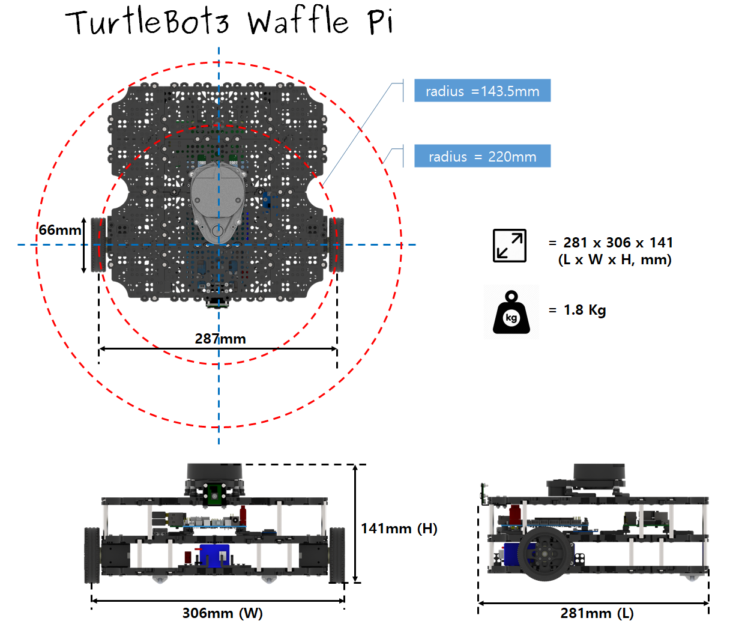
\includegraphics[height=0.60\textheight]{figs/tb3/turtlebot3_dimension3.png}
    \caption{Turtlebot3 Waffle Pi Dimensions and Mass}
    \label{fig:turtlebot3_dimensions}
\end{figure}
\begin{figure}[!h]
    \centering
    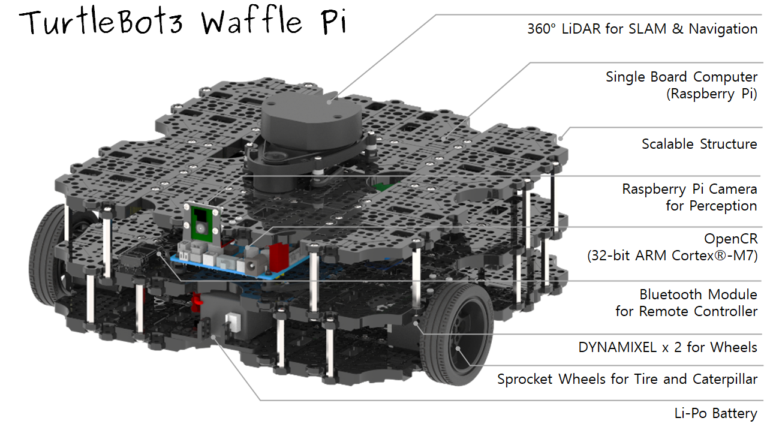
\includegraphics[width=0.90\textwidth]{figs/tb3/turtlebot3_waffle_pi_components.png}
    \caption{Turtlebot3 Waffle Pi Components (Note: The LiDAR sensor shown in this figure is not used in this project, as we employ pure vision-based SLAM)}
    \label{fig:turtlebot3_components}
\end{figure}
For more detailed specifications and component lists of Turtlebot3 Waffle Pi, please refer to Appendix~\ref{sec:turtlebot3_details}.

\subsection{Stereo Vision Camera -- ZED 2}
ZED 2 is a high-performance stereo vision camera, used for visual SLAM and environment perception. Its front view is shown in Figure~\ref{fig:zed2_camera}.
\begin{figure}[htbp]
    \centering
    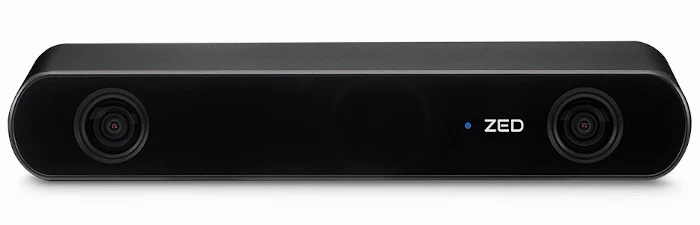
\includegraphics[width=0.9\textwidth]{figs/zed2/ZED-2-front.png}
    \caption{ZED 2 Stereo Vision Camera}
    \label{fig:zed2_camera}
\end{figure}
For more detailed specifications of ZED 2, please refer to Appendix~\ref{sec:zed2_details}.

\subsection{Edge Computing Unit -- Jetson Orin Nano}
Regarding the selection of the edge computing unit, NVIDIA has released various configurations of single\-board computers, including 4GB, 8GB, 16GB, 32GB, 64GB, and 128GB. Considering the actual requirements of this project, we chose the Jetson Orin Nano 8GB version. It is a lightweight embedded edge computing single\-board computer launched by NVIDIA, suitable for AI inference and edge computing tasks. Its layout diagram is shown in Figure~\ref{fig:jetson_orin_nano_layout}, and its components are listed in Table~\ref{tab:jetson_orin_nano_components}.

    \begin{figure}[h]
        \centering
        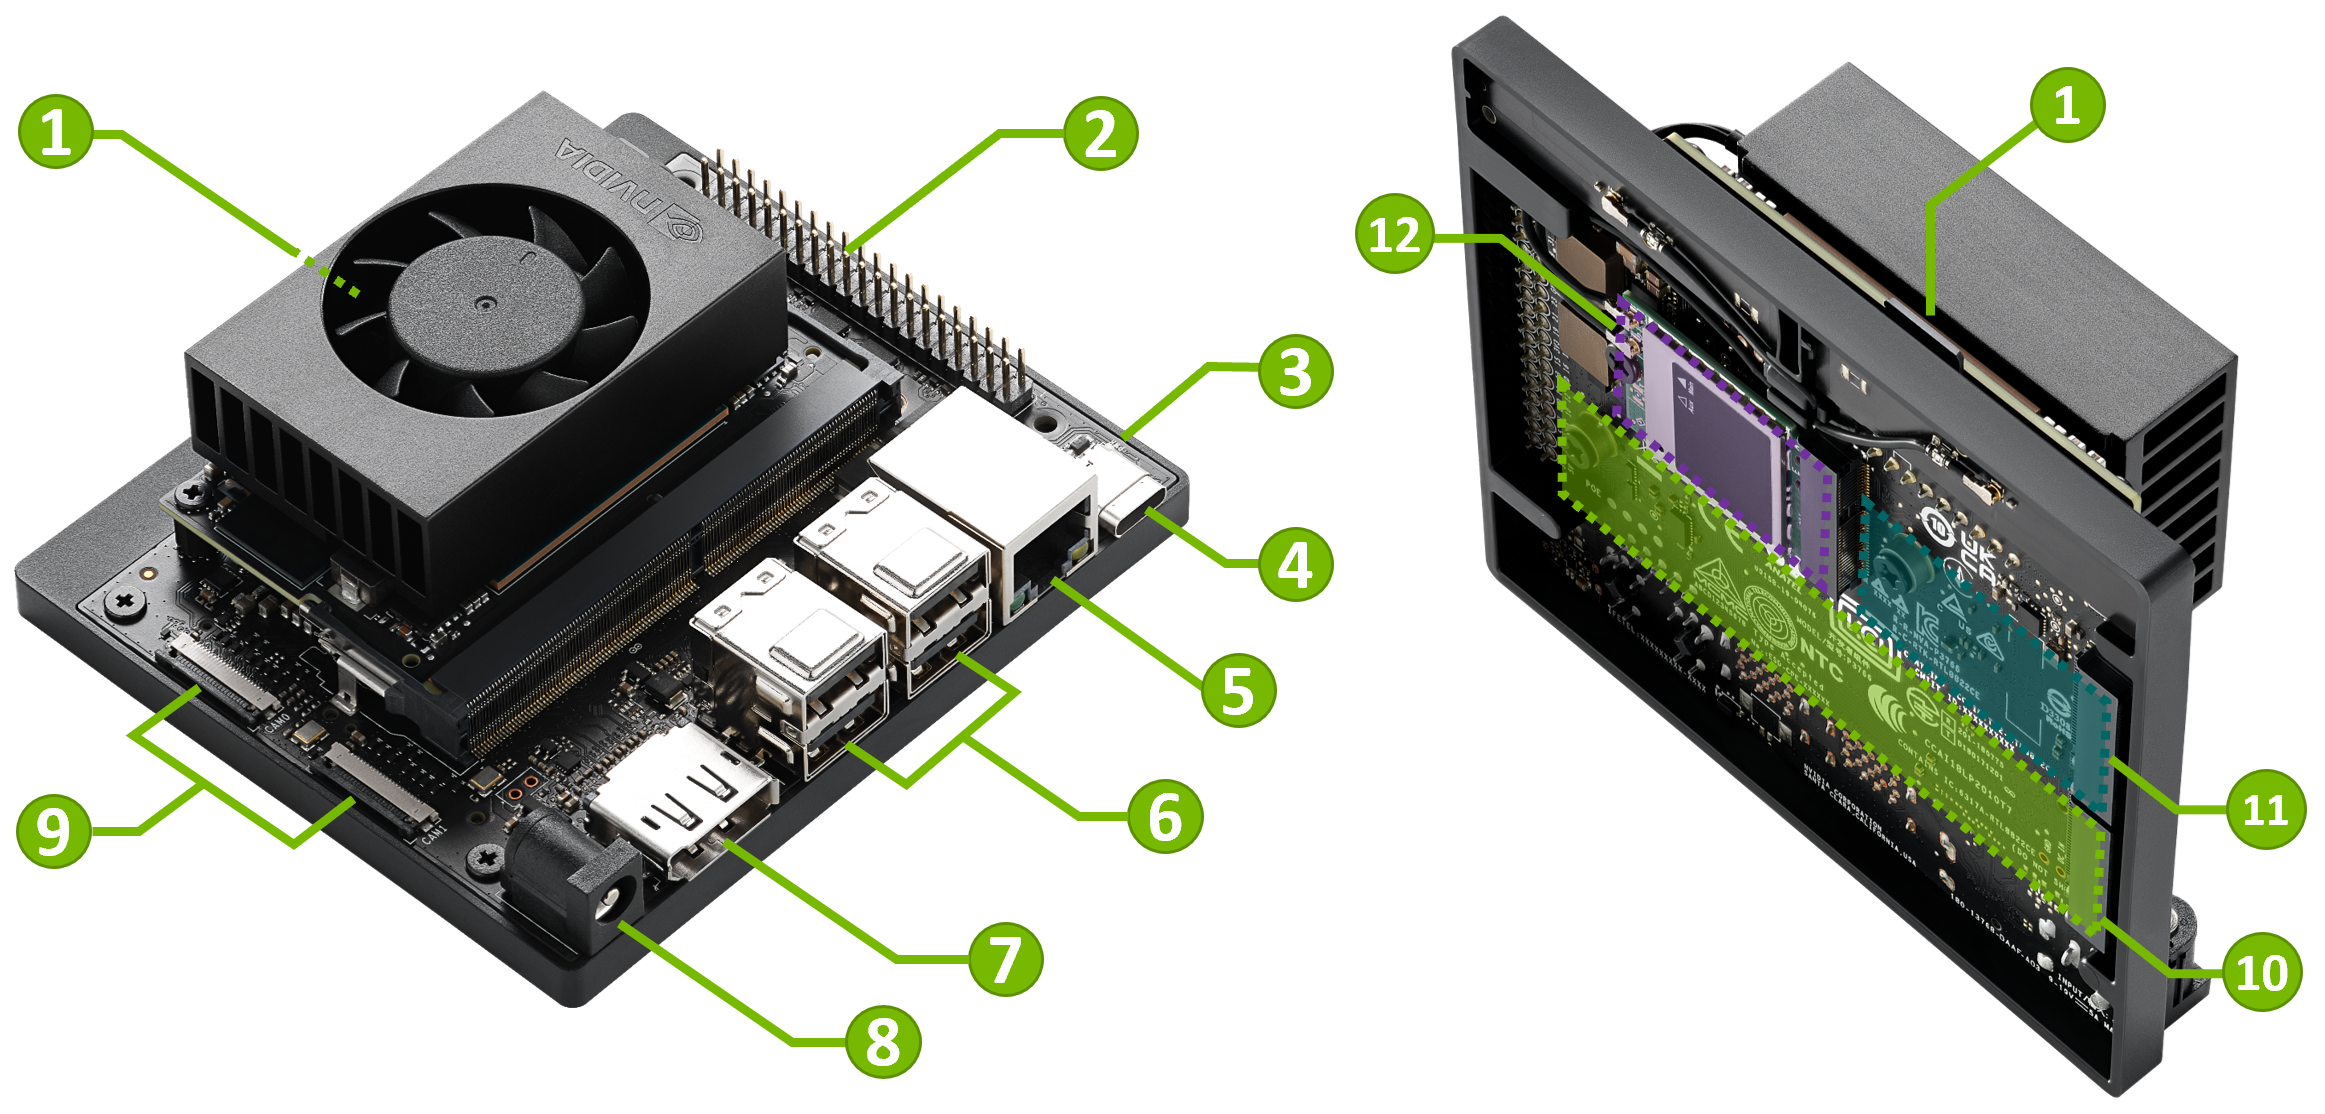
\includegraphics[width=0.9\textwidth]{figs/orin/jetson-nano-dev-kit_2view_numbered.png}
        \caption{Jetson Orin Nano Layout Diagram}
        \label{fig:jetson_orin_nano_layout}
    \end{figure}
    \begin{table}[h]
        \centering
        \caption{Jetson Orin Nano Components}
        \label{tab:jetson_orin_nano_components}
        \begin{tabular}{|c|l|p{6cm}|}
            \hline
            \textbf{Mark} & \textbf{Name} & \textbf{Note} \\
            \hline
            1 & microSD card slot & \\
            \hline
            2 & 40-pin Expansion Header & \\
            \hline
            3 & Power Indicator LED & \\
            \hline
            4 & USB-C port & For data only \\
            \hline
            5 & Gigabit Ethernet Port & \\
            \hline
            6 & USB 3.2 Type-A ports (x4) & 10Gbps \\
            \hline
            7 & DisplayPort Output Connector & \\
            \hline
            8 & DC Power Jack & 5.5mm x 2.5mm \\
            \hline
            9 & MIPI CSI Camera Connectors (x2) & 22pin, 0.5mm pitch \\
            \hline
            10 & M.2 Slot (Key-M, Type 2280) & PCIe 3.0 x4 \\
            \hline
            11 & M.2 Slot (Key-M, Type 2230) & PCIe 3.0 x2 \\
            \hline
            12 & M.2 Slot (Key-E, Type 2230) & (populated) \\
            \hline
        \end{tabular}
    \end{table}

\subsection{Power Supply -- INIU Power Bank}
 When selecting a power bank to supply power to the Jetson Orin Nano, we considered stability and chose a product with a voltage of up to 20V and a maximum output power of at least 65W. The INIU Power Bank was selected for this purpose. It has a capacity of 20000mAh and can output 65W at 20V, which is sufficient to power the Jetson Orin Nano. Its appearance is shown in Figure~\ref{fig:iniu_power_bank}.
\begin{figure}[htbp]
    \centering
    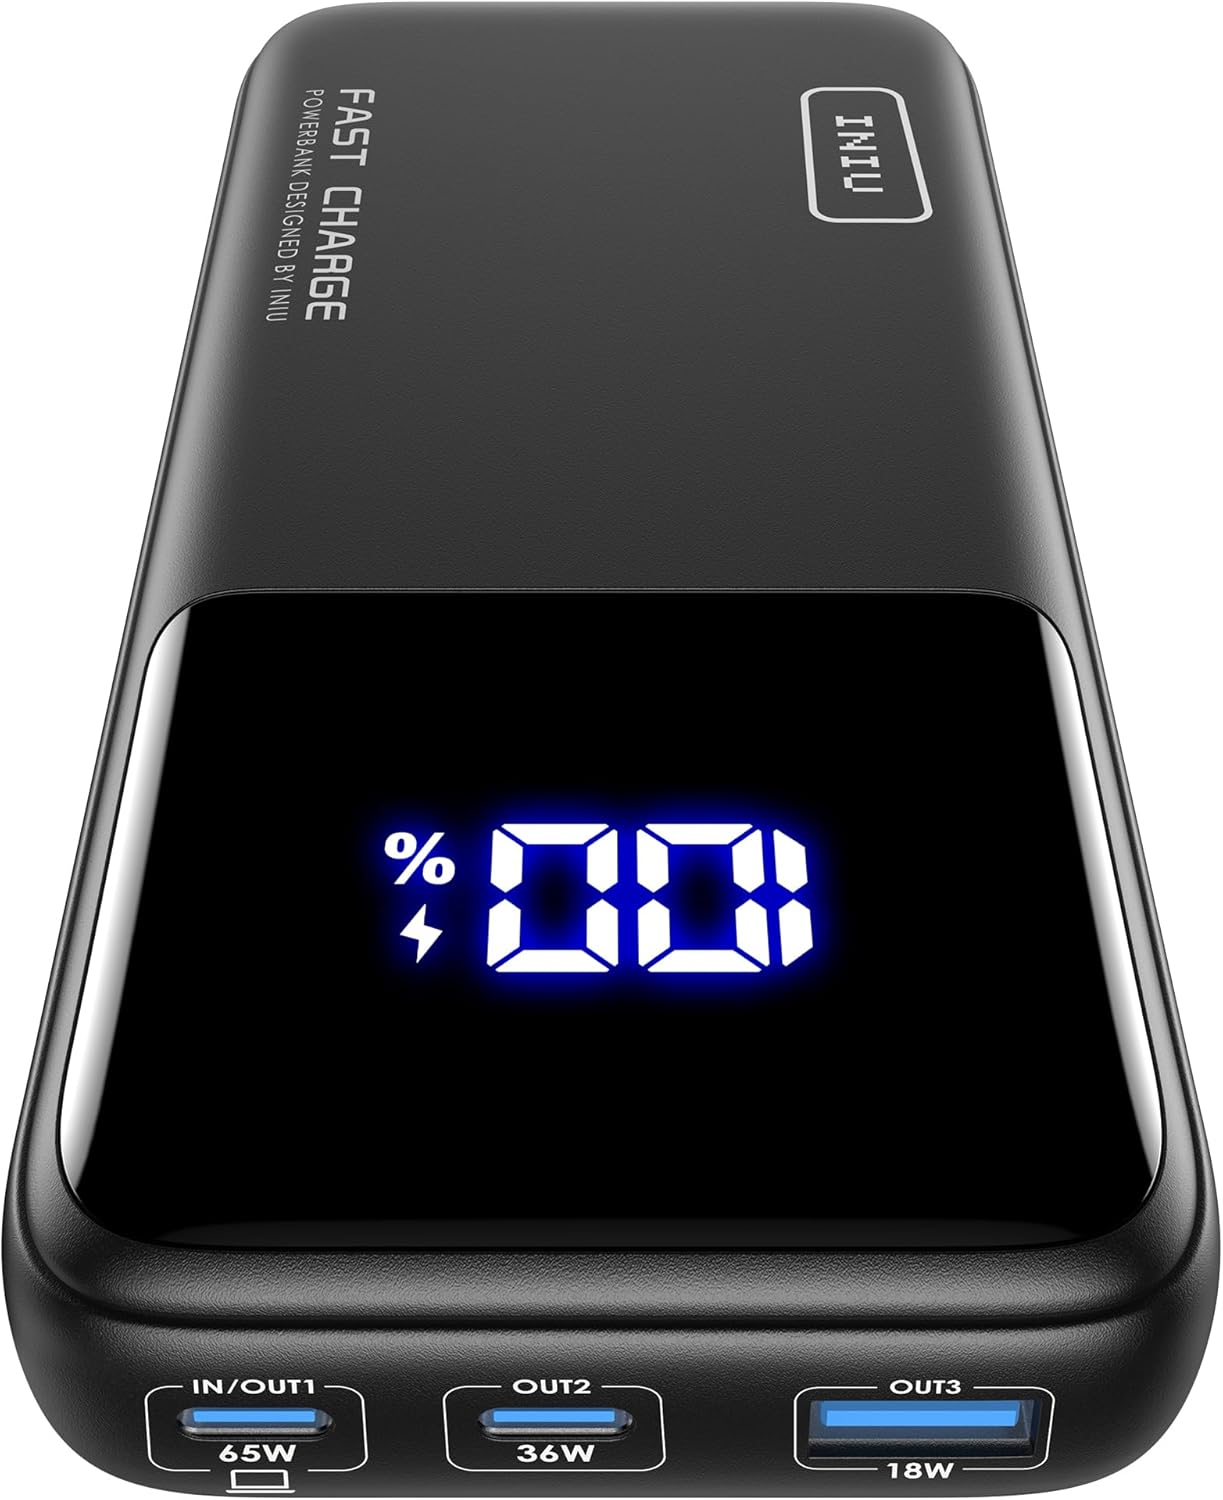
\includegraphics[width=0.5\textwidth]{figs/iniu/iniu_power_bank.jpg}
    \caption{INIU 65W 20000mAh Power Bank}
    \label{fig:iniu_power_bank}
\end{figure}
For more detailed specifications of INIU Power Bank, please refer to Appendix~\ref{sec:iniu_details}.

\subsection{Drone -- DJI Tello EDU}
To validate the feasibility of multi\-agent collaboration, this engineering selected the DJI Tello EDU drone. This drone is compact and lightweight, suitable for indoor flight and programming education. Its appearance is shown in Figure~\ref{fig:tello_edu_drone}. 

\begin{figure}[htbp]
    \centering
    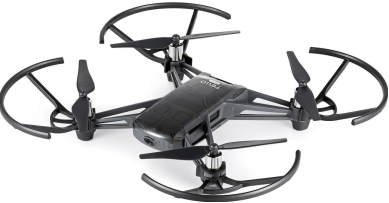
\includegraphics[width=0.5\textwidth]{figs/tello/tello_edu_drone.png}
    \caption{DJI Tello EDU Drone}
    \label{fig:tello_edu_drone}
\end{figure}
For more detailed specifications of DJI Tello EDU, please refer to Appendix~\ref{sec:tello_details}.

\subsection{Monitoring System -- Lenovo Laptop Yoga 14s 2021}
The monitoring system for this project uses a Lenovo laptop with 16GB of RAM, suitable for data processing and visualization tasks. 
For more detailed specifications of Lenovo Laptop Yoga 14s 2021, please refer to Appendix~\ref{sec:lenovo_details}.

\section{Environment Setup}
In this section, we will introduce how to set up the environment required for this engineering project, including the PC, Turtlebot3, and Jetson Orin Nano.

\subsection{PC Setup\label{subsec:pc_setup}}
This engineering project uses a standard laptop as the PC. The specific hardware configuration is shown in Table~\ref{tab:lenovo_laptop_specs}. On the PC, we mainly install the operating system, ROS 2, rtabmap package, the engineering package \texttt{uoa\_robot\_drone} and the development environment VS Code, and perform the corresponding environment configuration. Below, we will detail these steps.

\subsubsection{\textbf{Installing the Operating System}\label{subsubsec:os_setup}}
This engineering project uses Ubuntu 22.04 LTS as the operating system. *Note: To avoid issues, it is essential to install the OS using the \textbf{physical machine direct installation} method, not in a virtual machine (as Ubuntu on a virtual machine often fails during the Jetson Orin Nano flashing process). The installation steps are as follows:
\begin{enumerate}
    \item Click on the link https://releases.ubuntu.com/22.04/ to download the ISO image file of Ubuntu 22.04 LTS, as shown in Figure~\ref{fig:download_ubuntu_desktop}.
        \begin{figure}[!h]
            \centering
            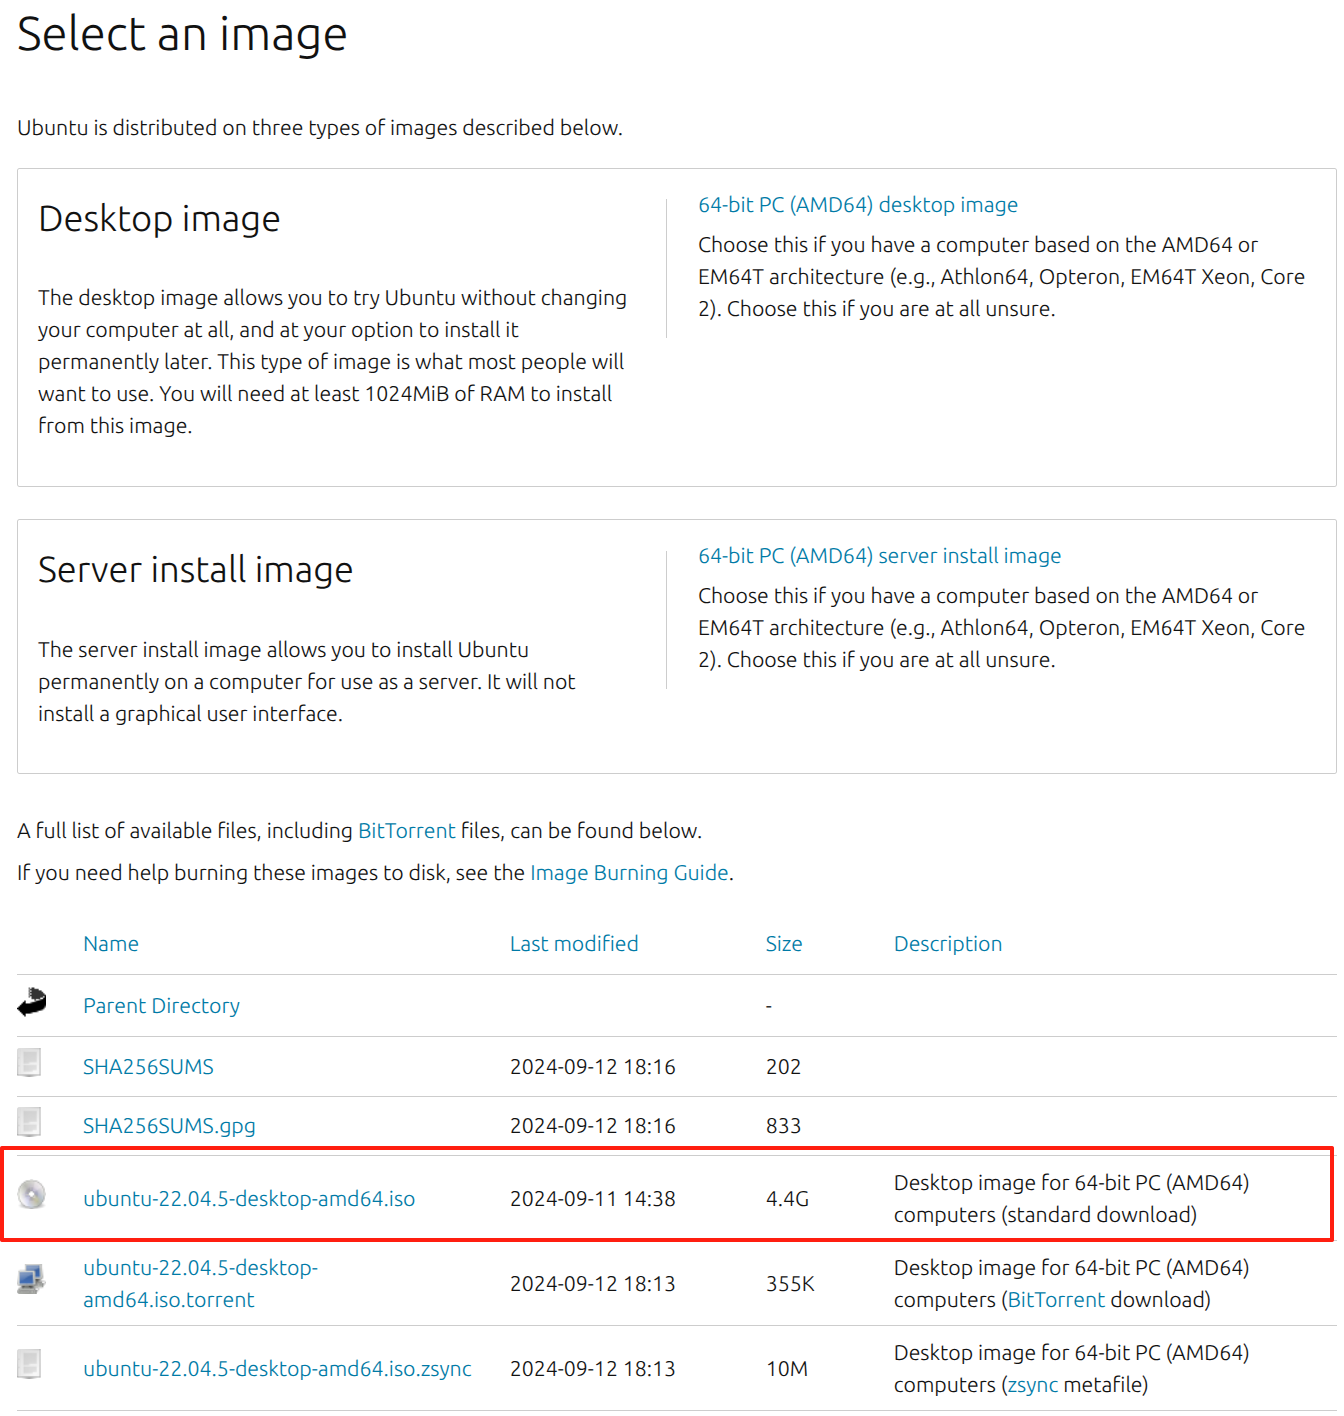
\includegraphics[width=0.9\textwidth]{figs/implementation/download_ubuntu_desktop.png}
            \caption{Downloading the ISO Image File of Ubuntu 22.04 LTS}
            \label{fig:download_ubuntu_desktop}
        \end{figure}
    \item Follow the tutorial \href{https://ubuntu.com/tutorials/install-ubuntu-desktop#1-overview}{Install Ubuntu Desktop} to complete the OS installation, as shown in Figure~\ref{fig:install_ubuntu_desktop}.
        \begin{figure}[!h]
            \centering
            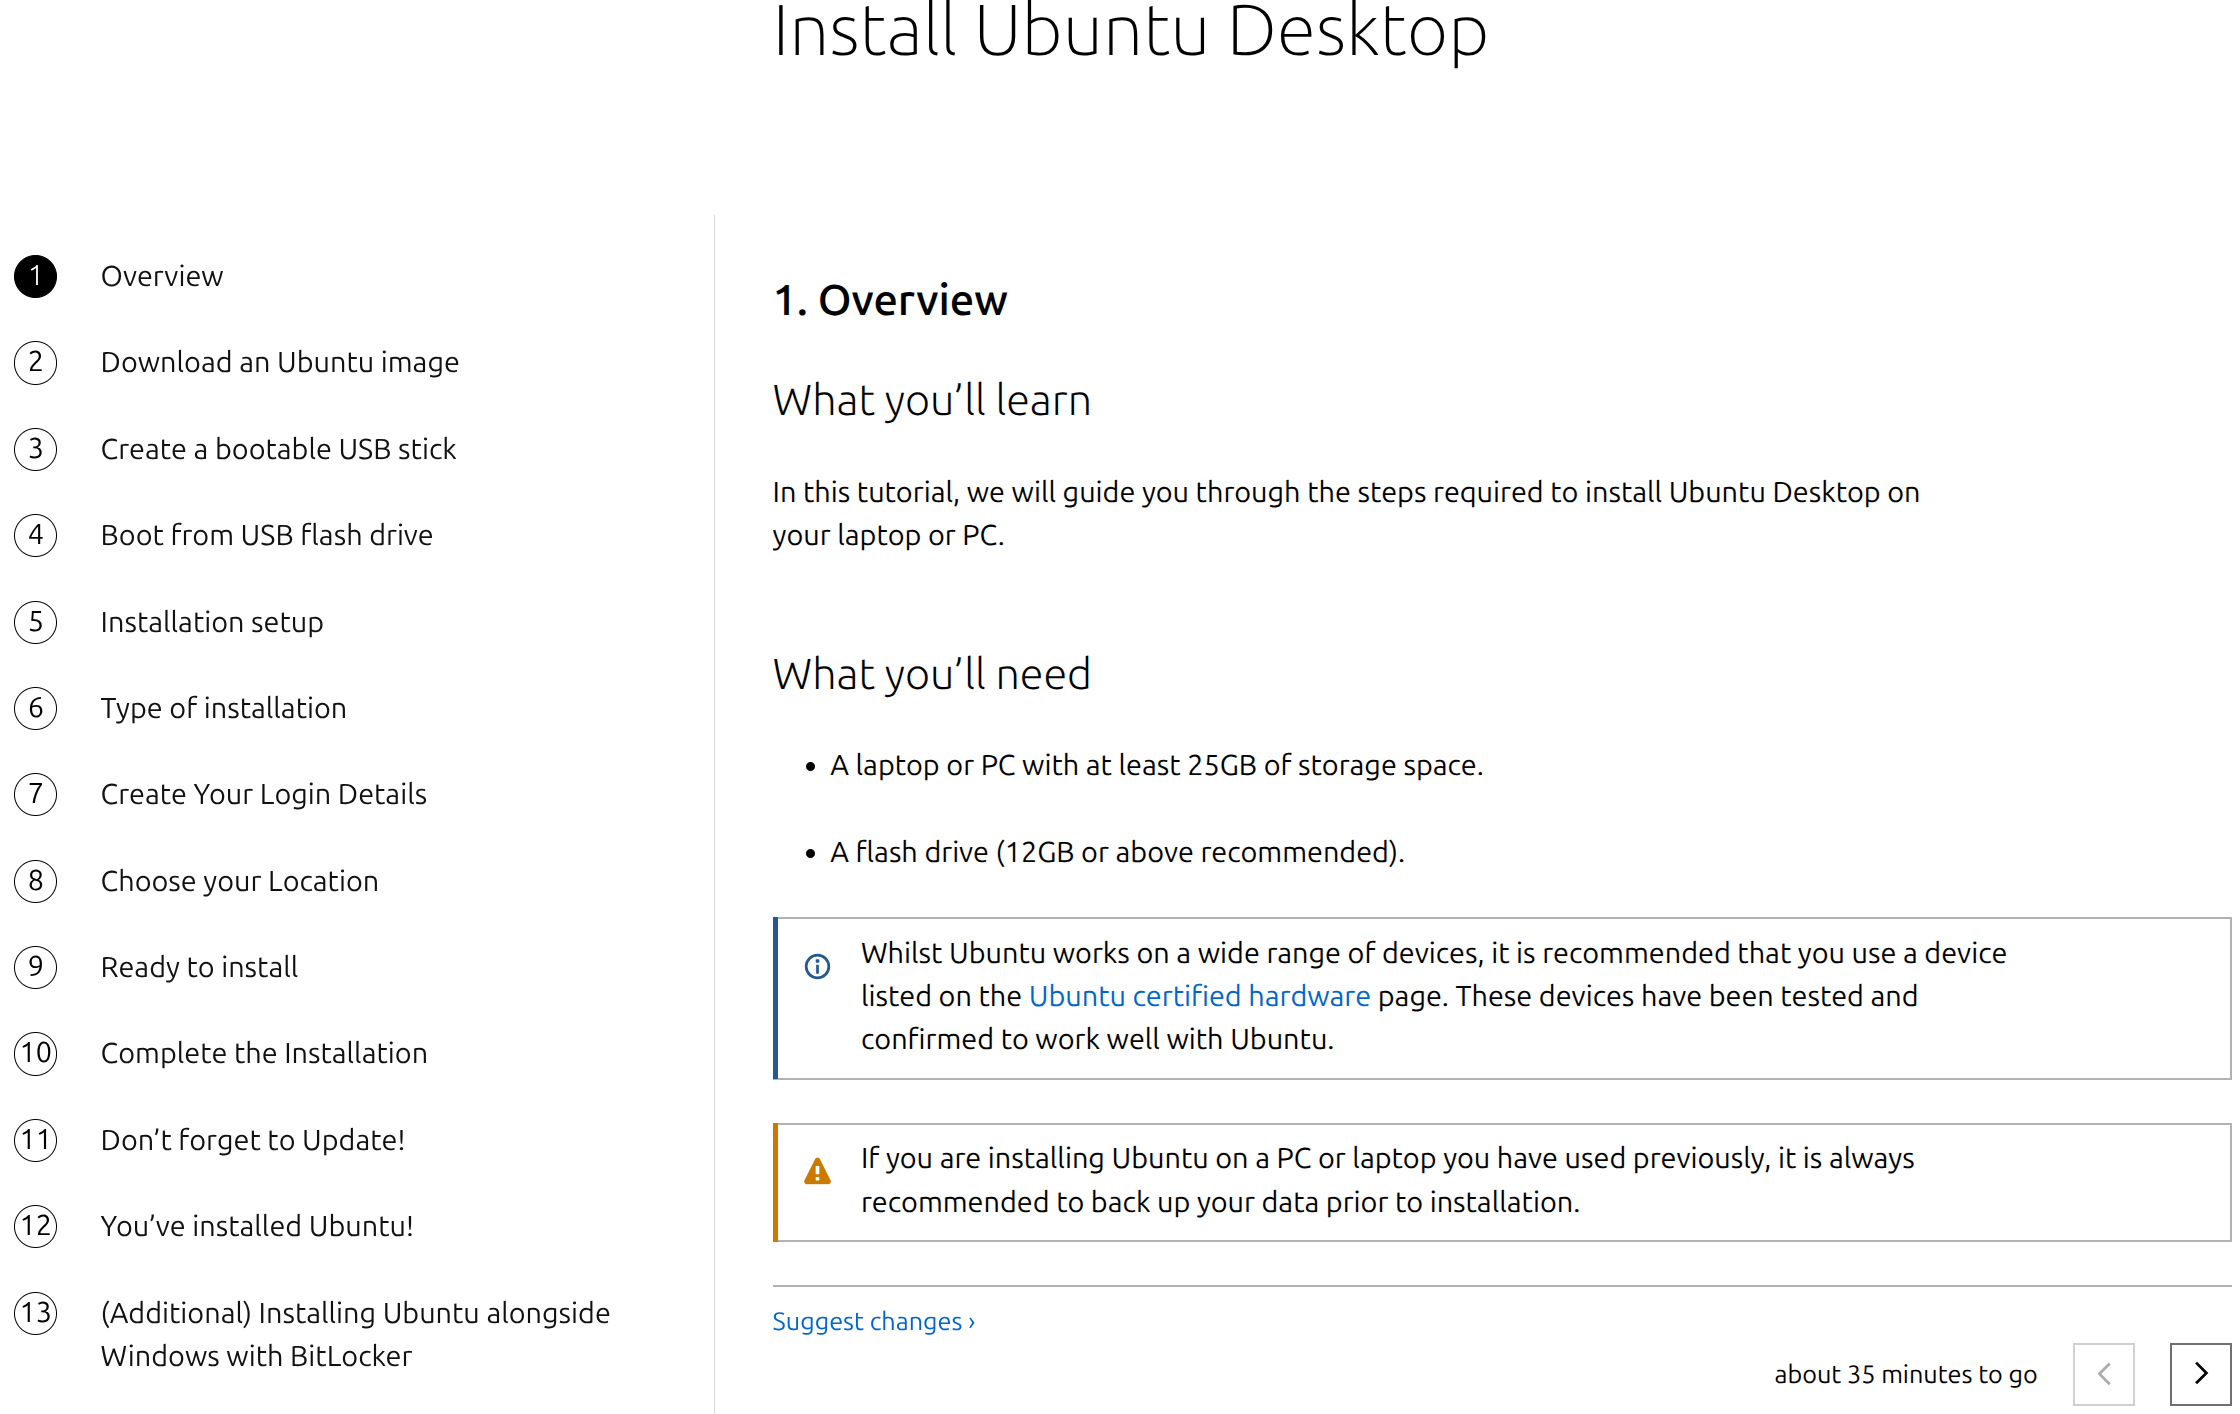
\includegraphics[width=0.9\textwidth]{figs/implementation/install_ubuntu_desktop.png}
            \caption{Installing Ubuntu 22.04 LTS}
            \label{fig:install_ubuntu_desktop}
        \end{figure}
\end{enumerate}

\subsubsection{\textbf{Installing ROS 2}\label{subsubsec:ros_setup}}
This engineering project uses ROS 2 Humble Hawksbill as the version. Follow the tutorial \href{https://docs.ros.org/en/humble/Installation/Ubuntu-Install-Debs.html}{Ubuntu (deb packages)} to install step by step, and execute the steps shown in Figure~\ref{fig:try_some_examples}.
\begin{figure}[!h]
    \centering
    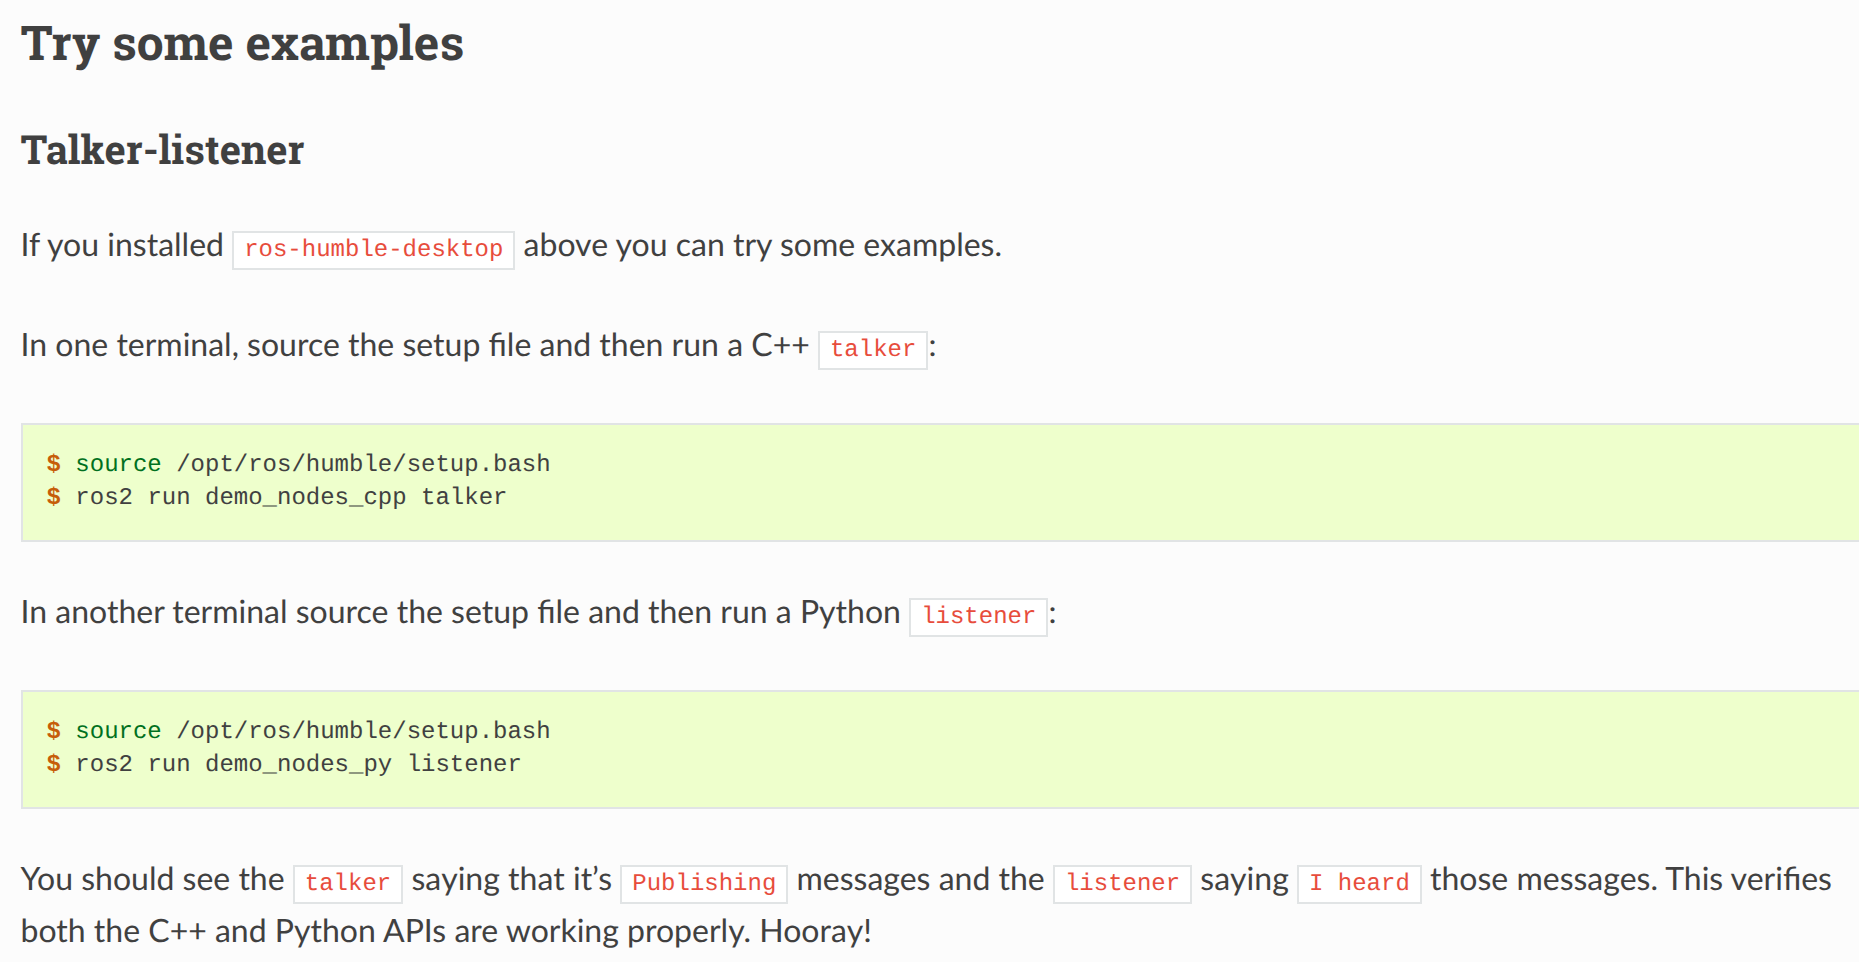
\includegraphics[width=0.9\textwidth]{figs/implementation/try_some_examples.png}
    \caption{Installing ROS 2 Humble Hawksbill}
    \label{fig:try_some_examples}
\end{figure}   

\subsubsection{\textbf{Installing Packages}\label{subsubsec:packages_setup}}
On the PC, the main packages used in this engineering project are Turtlebot3, rtabmap, and navigation2.
[On PC] The relevant installation commands are as follows:
\begin{lstlisting}[language=bash]
$ source /opt/ros/humble/setup.bash
$ mkdir -p ~/ros2_ws/src
$ cd ~/ros2_ws/src/
$ git clone -b humble https://github.com/ROBOTIS-GIT/DynamixelSDK.git
$ git clone -b humble https://github.com/ROBOTIS-GIT/turtlebot3_msgs.git
$ git clone -b humble https://github.com/ROBOTIS-GIT/turtlebot3.git
$ git clone https://github.com/introlab/rtabmap.git
$ git clone -b ros2 https://github.com/introlab/rtabmap_ros.git
$ git clone -b humble https://github.com/ros-navigation/navigation2.git
$ git clone -b humble https://github.com/Jian-UOA/CS5917.git
$ sudo apt install python3-colcon-common-extensions
$ cd ~/ros2_ws
$ colcon build --symlink-install
\end{lstlisting}

\subsubsection{\textbf{Installing the Development Environment}\label{subsubsec:dev_env_setup}}
This engineering project uses Visual Studio Code as the development environment. The installation steps are as follows:
\begin{enumerate}
    \item Click on the link https://code.visualstudio.com/Download to download the appropriate version of Visual Studio Code (in this engineering project, the x64 version is selected), as shown in Figure~\ref{fig:download_vscode}.
        \begin{figure}[!h]
            \centering
            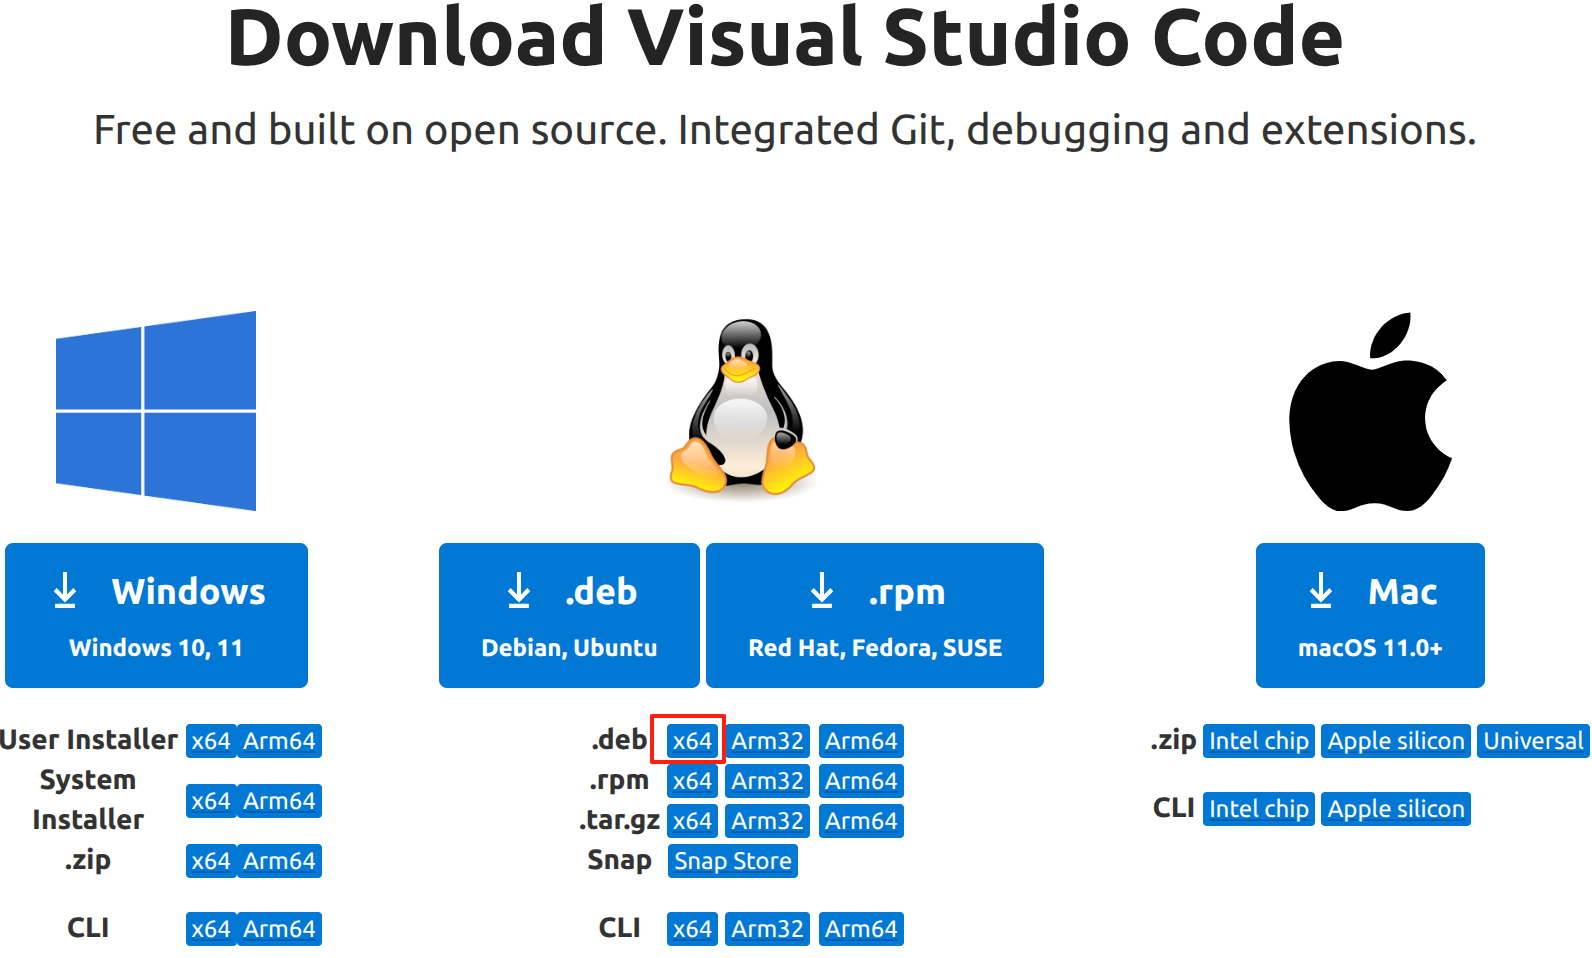
\includegraphics[width=0.9\textwidth]{figs/implementation/download_vscode.png}
            \caption{Downloading Visual Studio Code}
            \label{fig:download_vscode}
        \end{figure}
    \item Go to the directory where the downloaded file is saved, find the downloaded installation file (\texttt{code\_1.103.1-1755017277\_amd64.deb}), and follow the tutorial \href{https://code.visualstudio.com/docs/setup/linux#_install-vs-code-on-linux}{Install VS Code on Linux} to complete the installation, as shown in Figure~\ref{fig:install_vscode}.
        \begin{figure}[!h]
            \centering
            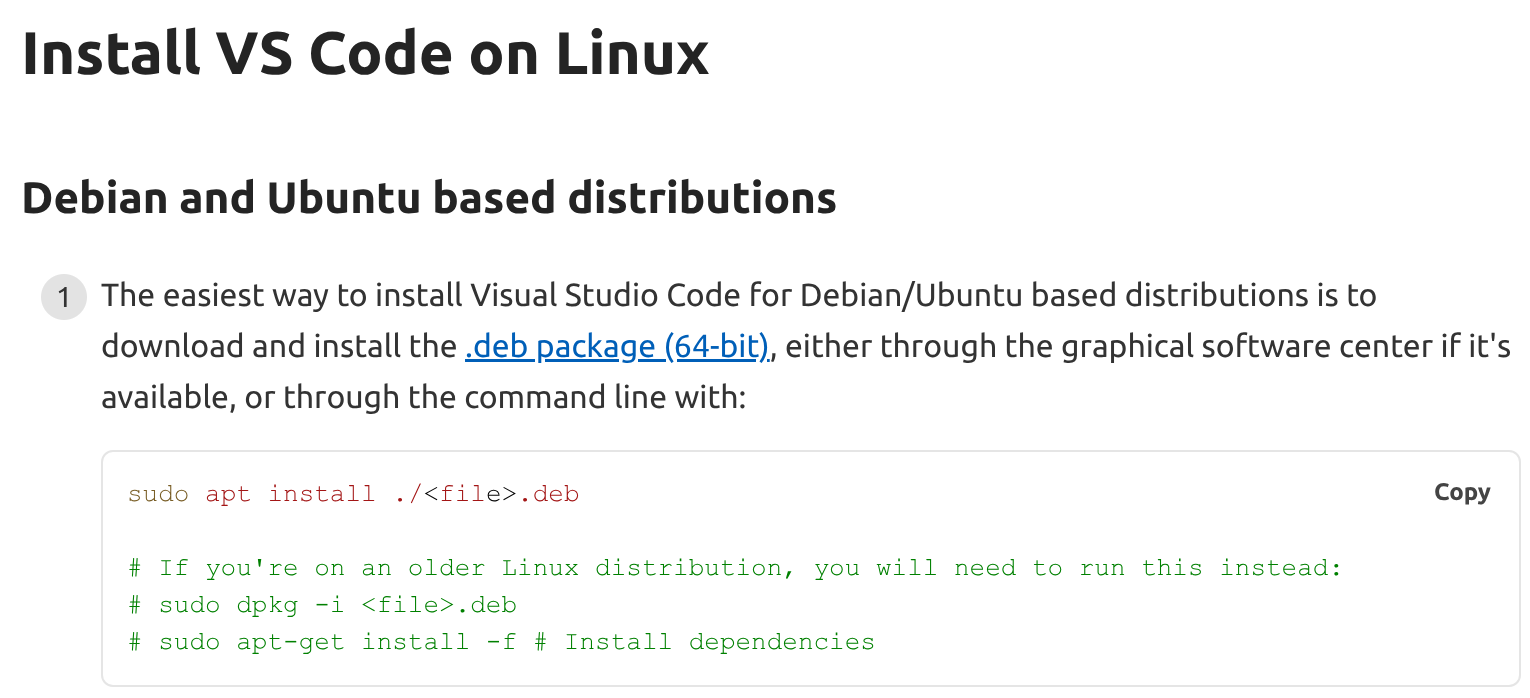
\includegraphics[width=0.9\textwidth]{figs/implementation/install_vscode.png}
            \caption{Installing Visual Studio Code}
            \label{fig:install_vscode}
        \end{figure}
    \item Open Visual Studio Code, follow the example in the tutorial \href{https://code.visualstudio.com/docs/getstarted/getting-started}{Tutorial: Get started with Visual Studio Code}, complete the basic configuration, and open the workspace in the directory \texttt{~/ros2\_ws}. You should see content similar to Figure~\ref{fig:open_ros2_ws}.
        \begin{figure}[!h]
            \centering
            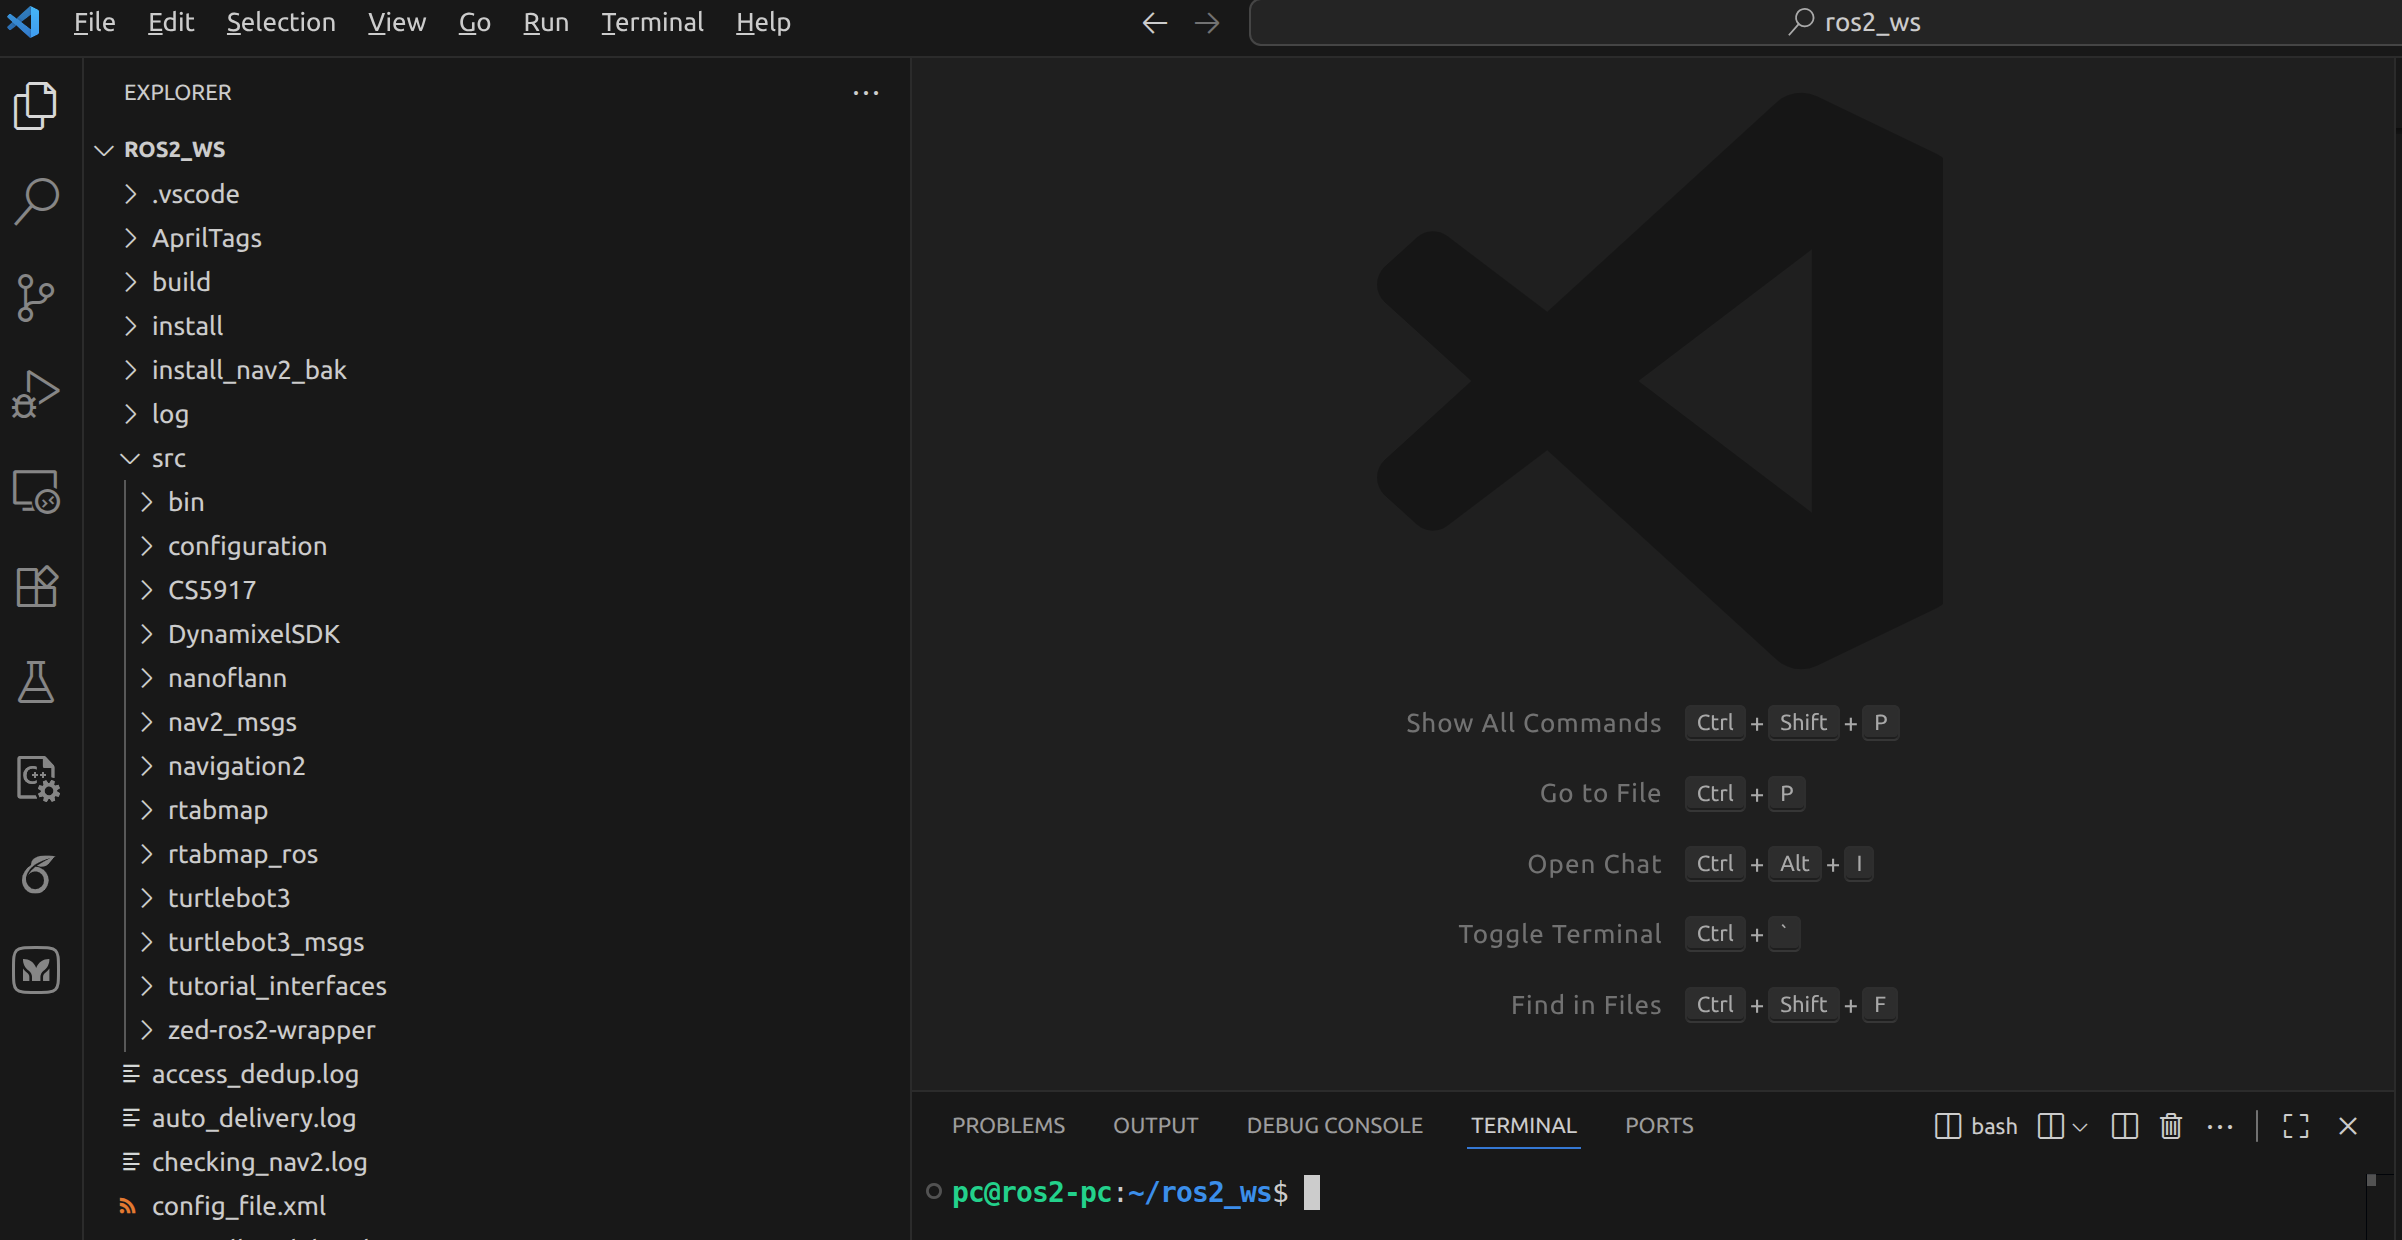
\includegraphics[width=0.9\textwidth]{figs/implementation/open_ros2_ws.png}
            \caption{Opening ROS 2 Workspace}
            \label{fig:open_ros2_ws}
        \end{figure}
\end{enumerate}

\subsubsection{\textbf{Environment Configuration}\label{subsubsec:env_setup}}
[On PC] The relevant configuration commands are as follows:
\begin{lstlisting}[language=bash]
$ echo 'source ~/ros2_ws/install/setup.bash' >> ~/.bashrc
$ echo 'source /opt/ros/humble/setup.bash' >> ~/.bashrc
$ echo "export TURTLEBOT3_MODEL=waffle_pi" >> ~/.bashrc
$ echo 'export ROS_DOMAIN_ID=30 #TURTLEBOT3' >> ~/.bashrc
$ echo 'export RMW_IMPLEMENTATION=rmw_fastrtps_cpp' >> ~/.bashrc
$ source ~/.bashrc
\end{lstlisting}

\subsection{Turtlebot3 Setup\label{subsec:turtlebot3_setup}}
This engineering project uses the Turtlebot3 Waffle Pi version. The specific hardware configuration is shown in Table~\ref{tab:turtlebot3_specs}. For the setup of the Single Board Computer (SBC) and OpenCR on Turtlebot3, please refer to the tutorials \href{https://emanual.robotis.com/docs/en/platform/turtlebot3/sbc_setup/#sbc-setup}{SBC Setup} and \href{https://emanual.robotis.com/docs/en/platform/turtlebot3/opencr_setup/#opencr-setup}{OpenCR Setup}.

\subsection{Jetson Orin Nano Setup\label{subsec:jetson_orin_nano_setup}}
This engineering project uses the Jetson Orin Nano Developer Kit version. The specific hardware configuration is shown in Table~\ref{tab:jetson_orin_nano_specs}. On the Jetson Orin Nano, we mainly install the operating system, ROS 2, ZED SDK, ZED package, rtabmap package, and the engineering package \texttt{uoa\_robot\_drone}, and perform the corresponding environment configuration. Below, we will detail these steps.

\subsubsection{\textbf{Installing the Operating System}\label{subsubsec:jetson_os_setup}}
\begin{enumerate}
    \item After registering a free account according to the tutorial \href{https://docs.nvidia.com/sdk-manager/download-run-sdkm/index.html}{Download and Run SDK Manager}, use the SDK Manager to install Jet Pack version 6.2.1.
    \item Access the graphical interface of the Jetson Orin Nano's Ubuntu system and connect to a wireless network.
    \item To save resources, SSH into the Jetson Orin Nano and enter the command:
    \begin{lstlisting}[language=bash]
        ssh username@ip_address
    \end{lstlisting}
    where \texttt{username} is the username of the Jetson Orin Nano, and \texttt{ip\_address} is the IP address of the Jetson Orin Nano.
    \item After entering the Ubuntu system of the Jetson Orin Nano, enter the command:
    \begin{lstlisting}[language=bash]
        sudo systemctl set-default multi-user.target
        sudo systemctl reboot
    \end{lstlisting}
    \item After rebooting, the Jetson Orin Nano will enter command line mode.
\end{enumerate}

\subsubsection{\textbf{Installing ROS 2}\label{subsubsec:jetson_ros_setup}}
This engineering project uses ROS 2 Humble Hawksbill as the version. Follow the tutorial \href{https://docs.ros.org/en/humble/Installation/Ubuntu-Install-Debs.html}{Ubuntu (deb packages)} to install step by step, and execute the steps shown in Figure~\ref{fig:try_some_examples}.

\subsubsection{\textbf{Installing ZED SDK}\label{subsubsec:zed_sdk_setup}}
This engineering project uses the CUDA 12 ZED SDK for Ubuntu 22 version 5.0. Follow the tutorial \href{https://www.stereolabs.com/docs/development/zed-sdk/linux}{Download and Install the ZED SDK} to install step by step. It is not recommended to install in \texttt{silent mode}.

\subsubsection{\textbf{Installing Packages}\label{subsubsec:jetson_packages_setup}}
On the Jetson Orin Nano, the main packages used in this engineering project are the ZED 2 stereo camera, rtabmap, and the engineering package \texttt{uoa\_robot\_drone}.
[On Jetson Orin Nano] The relevant installation commands are as follows:
\begin{lstlisting}[language=bash]
$ source ~/.bashrc
$ mkdir -p ~/colcon_ws/src
$ cd ~/colcon_ws
$ git clone https://github.com/stereolabs/zed-ros2-wrapper.git src/zed-ros2-wrapper 
$ git clone https://github.com/introlab/rtabmap.git src/rtabmap 
$ git clone -b ros2 https://github.com/introlab/rtabmap_ros.git src/rtabmap_ros
$ git clone -b humble https://github.com/Jian-UOA/CS5917.git src/CS5917
$ sudo apt install python3-colcon-common-extensions
$ colcon build --symlink-install
\end{lstlisting}

\subsubsection{\textbf{Environment Configuration}\label{subsubsec:jetson_env_setup}}
[On Jetson Orin Nano] The relevant configuration commands are as follows:
\begin{lstlisting}[language=bash]
$ echo 'source ~/colcon_ws/install/setup.bash' >> ~/.bashrc
$ echo 'source /opt/ros/humble/setup.bash' >> ~/.bashrc
$ echo 'export ROS_DOMAIN_ID=30' >> ~/.bashrc
$ echo 'export RMW_IMPLEMENTATION=rmw_fastrtps_cpp' >> ~/.bashrc
$ source ~/.bashrc
\end{lstlisting}

\subsubsection{\textbf{Verifying Installation}\label{subsubsec:jetson_verify_setup}}
To verify whether the installation on the Jetson Orin Nano was successful, follow these steps:
\begin{enumerate}
    \item Verify that the ZED 2 camera is successfully installed
        \begin{enumerate}
            \item Open a terminal on the PC, SSH into the Jetson Orin Nano, and enter the command:
                \begin{lstlisting}[language=bash]
                    $ clear && cd ~/colcon_ws && ros2 launch zed_wrapper zed_camera.launch.py | tee zed.log
                \end{lstlisting}
            \item If the ZED-related installation is successful, you should see output similar to Figure~\ref{fig:zed_camera_launch}.
                \begin{figure}[!h]
                    \centering
                    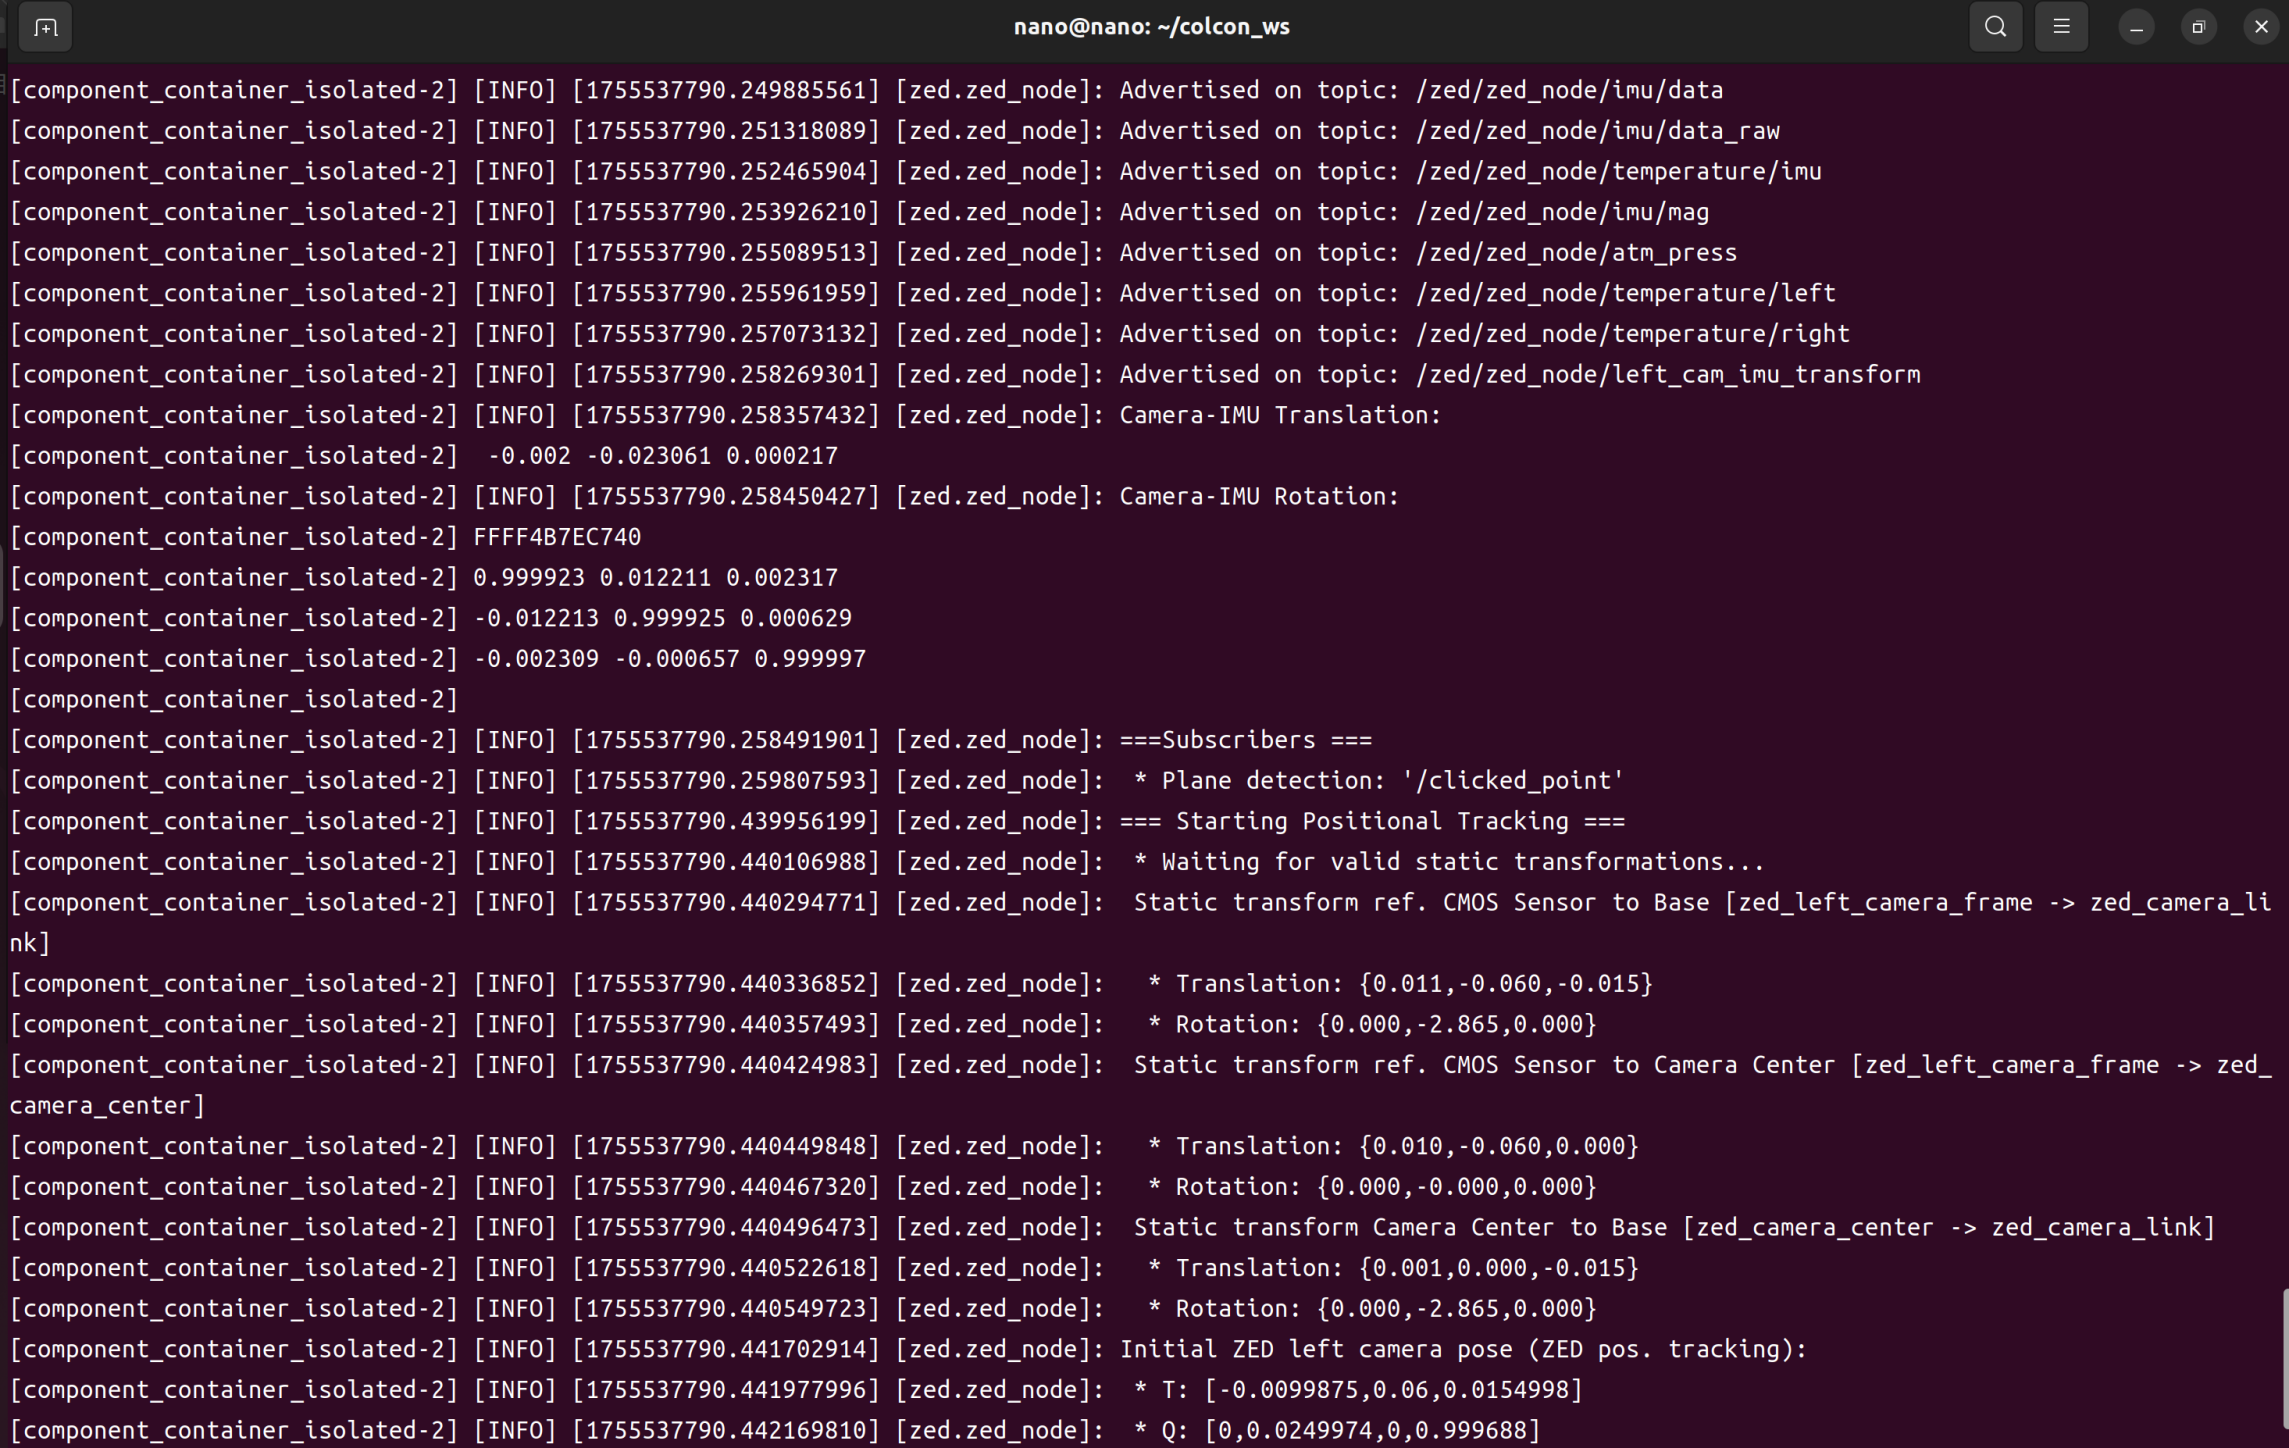
\includegraphics[width=0.9\textwidth]{figs/zed2/zed_camera_launch.png}
                    \caption{ZED Camera Launch Output}
                    \label{fig:zed_camera_launch}
                \end{figure} 
        \end{enumerate}
    \item Verify that the rtabmap package is successfully installed
        \begin{enumerate}
            \item On PC, press \texttt{Ctrl + Alt + T} to open a terminal, SSH into the Jetson Orin Nano, and enter the command:
                \begin{lstlisting}[language=bash]
                    $ clear && cd ~/colcon_ws && ros2 launch uoa_robot_drone orin_stereo_vslam.launch.py localization:=false | tee orin_vslam.log
                \end{lstlisting}
            \item If the rtabmap\-related installation is successful, you should see output similar to Figure~\ref{fig:orin_stereo_vslam_launch}.
                \begin{figure}[!h]
                    \centering
                    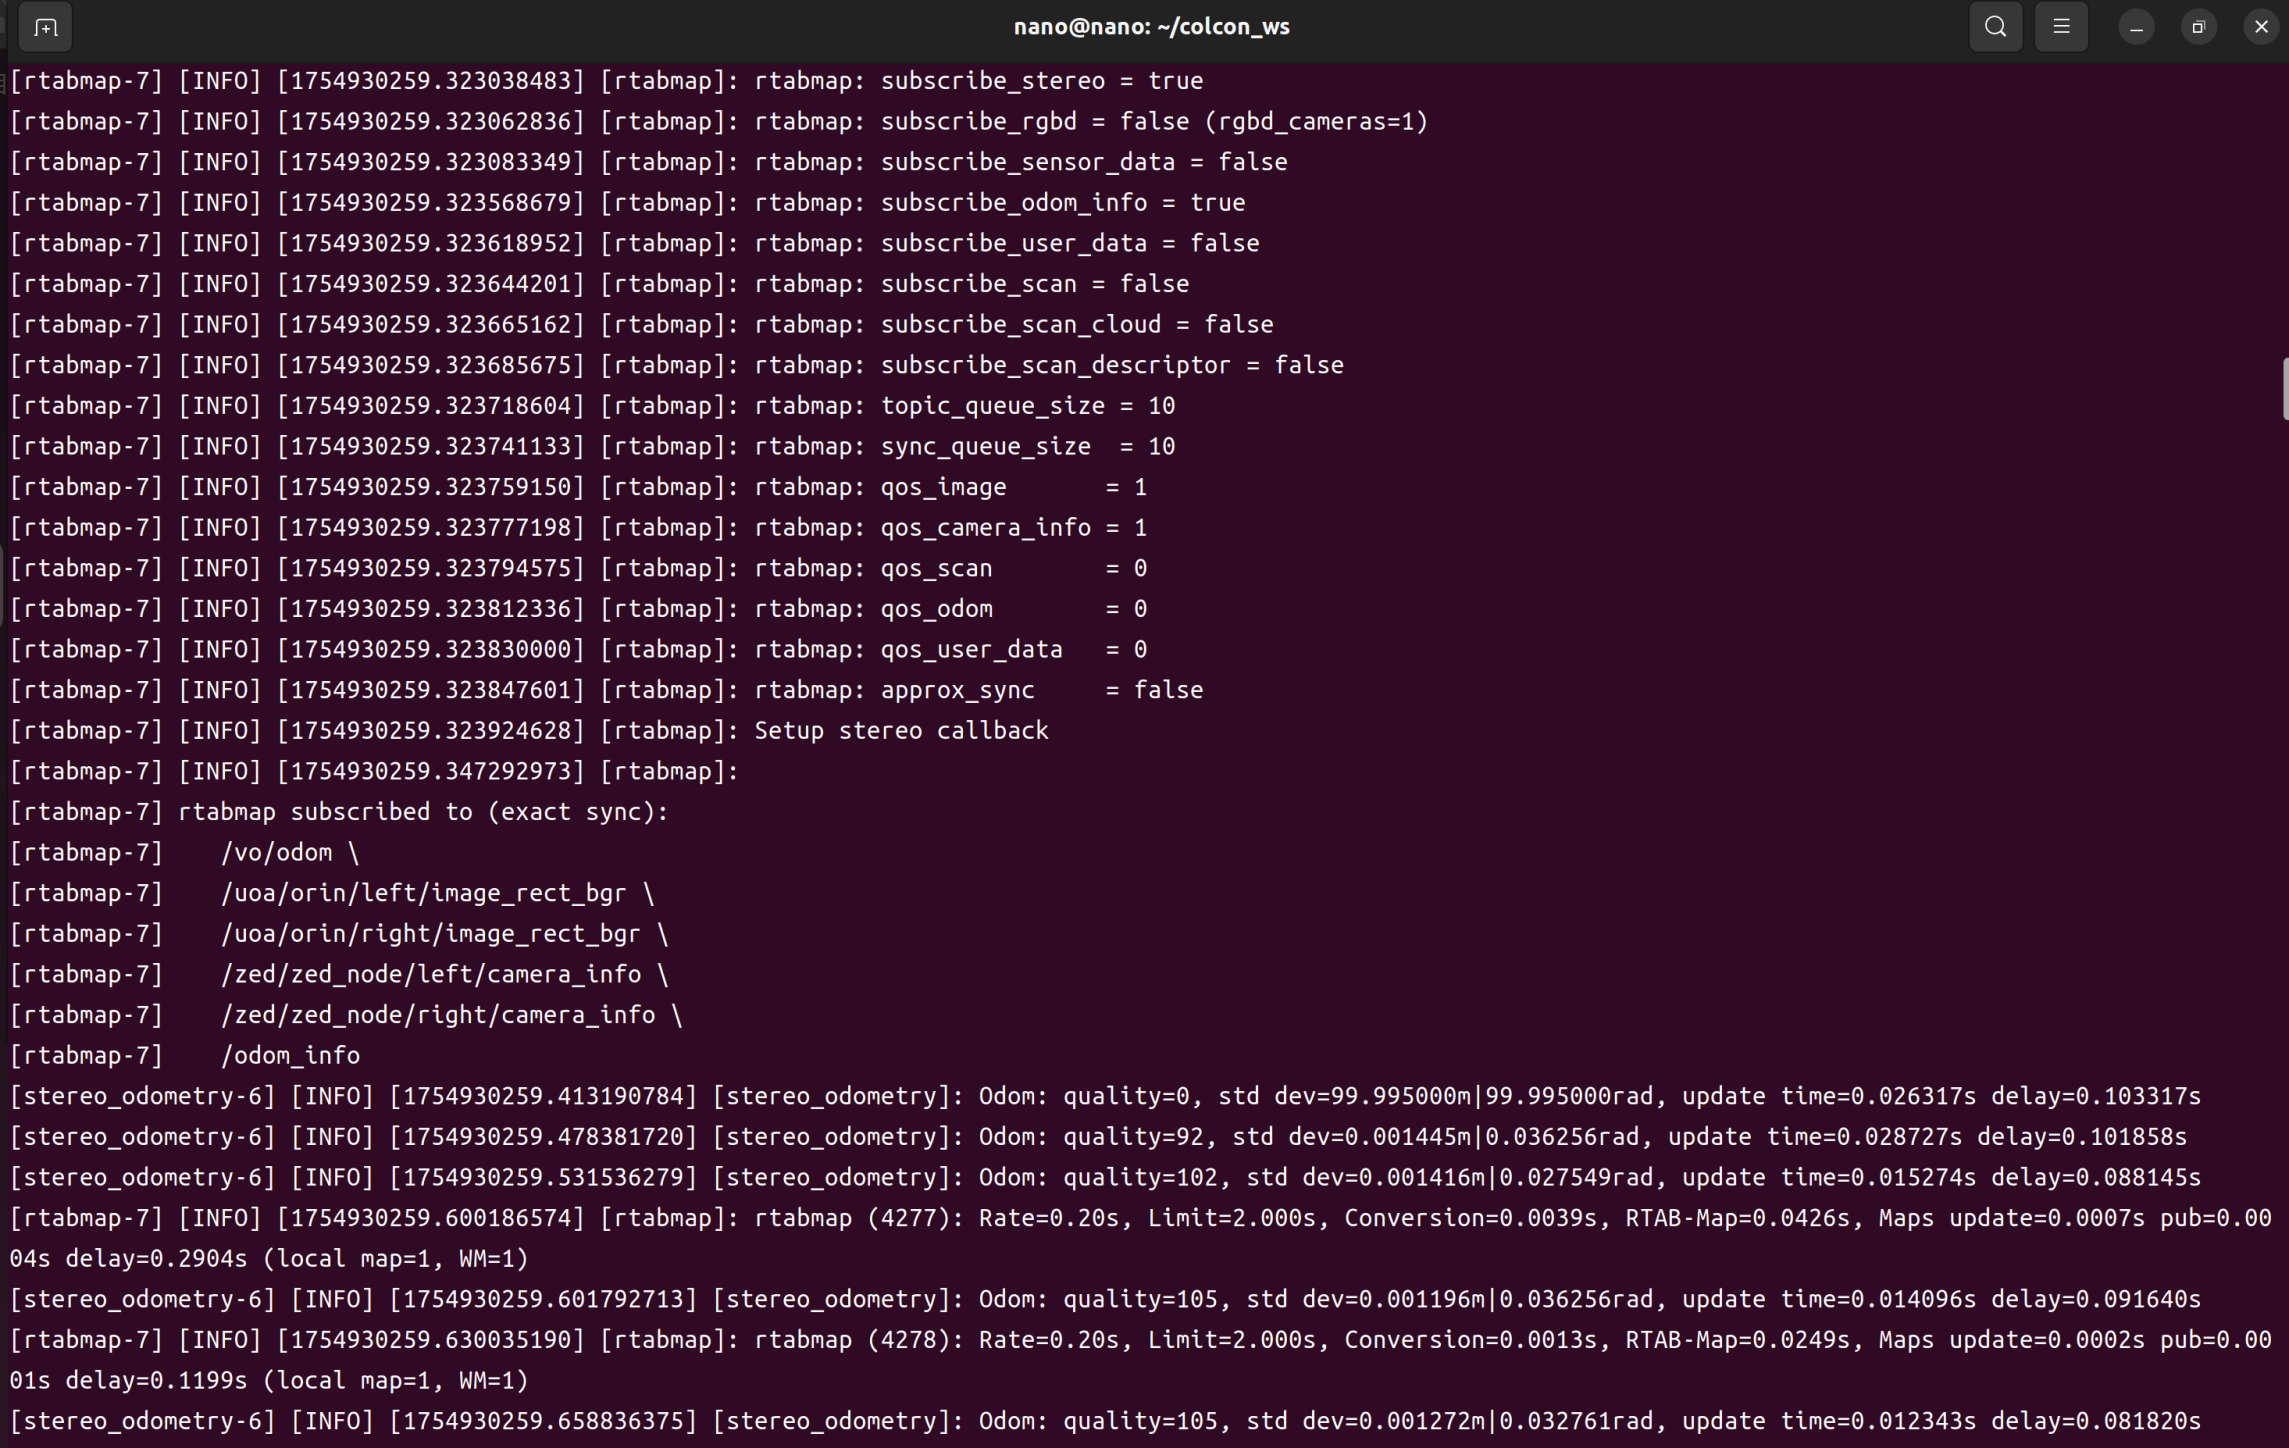
\includegraphics[width=0.9\textwidth]{figs/orin/orin_stereo_vslam_launch.png}
                    \caption{Orin Stereo Visual SLAM Launch Output}
                    \label{fig:orin_stereo_vslam_launch}
                \end{figure}
        \end{enumerate}
\end{enumerate}